	\documentclass[10pt,oneside]{CBFT_book}
	
	% Algunos paquetes
	
	\usepackage{amssymb}
	\usepackage{amsmath}
	\usepackage{graphicx}
	\usepackage{libertine}
	\usepackage{lipsum}
	\usepackage[numbers]{natbib}
	\setcitestyle{square}


	\usepackage{polyglossia}
	\setdefaultlanguage{spanish}

	\usepackage{CBFT.estilo} % Cargo la hoja de estilo
	
	% Tipografías
	% \setromanfont[Mapping=tex-text]{Linux Libertine O}
	% \setsansfont[Mapping=tex-text]{DejaVu Sans}
	% \setmonofont[Mapping=tex-text]{DejaVu Sans Mono}

	%===================================================================
	%	DOCUMENTO PROPIAMENTE DICHO
	%===================================================================

% \title{CBFT Mecánica clásica}
% \author{Mecánica lagrangiana}
% \date{\today}

\begin{document}
% \maketitle
% \tableofcontents
\chapter{Mecánica lagrangiana}

% =================================================================================================
\section{Principio de los trabajos virtuales}\index{Trabajos virtuales, principio de}
% =================================================================================================
\notamargen{Esto es sumamente sketchi, debemos leer la carpeta de la cursada y luego la
teoría.}

En las ecuaciones de Newton para un sistema de $N$ partículas, con $3N$ coordenadas,
\[
	m_i \vb{a}_i = \vb{F}_i,
\]
se pueden separar las fuerzas que actúan sobre cada partícula en fuerzas externas aplicadas $ \vb{F}_i^a $
y fuerzas de vínculo $ \vb{F}_i^v $. Es decir,
\[
	m_i \vb{a}_i = \vb{F}_i^a + \vb{F}_i^v,
\]
% dan cuenta de que sobre cada partícula actúan, en principio, fuerzas externas aplicadas $ \vb{F}_i^a $
% y fuerzas de vínculo $ \vb{F}_i^v $. 
o bien, expresando la aceleración en función de la derivada temporal del momento, 
%$ \dot{\vb{p}}_i = m_i \vb{a}_i$ 
resulta 
\[
	\dot{\vb{p}}_i - \vb{F}_i^a - \vb{F}_i^v = 0,
\]
y entonces, multiplicando cada término por un desplazamiento, en principio independiente, $ \delta\vb{x}_i $ y sumando se tiene
\[
	\sum_i^N \left( \dot{\vb{p}}_i - \vb{F}_i^a - \vb{F}_i^v \right) \cdot \delta\vb{x}_i  = 0.
\]
Nótese que esta ecuación es válida por serlo para cada partícula $i$.

\notamargen{Explicar qué es este principio y qué es un desplazamiento virtual.}
Supongamos ahora que estos desplazamientos son {\it compatibles} con los vínculos. Entonces
\[
	\sum_i^N \left( \dot{\vb{p}}_i - \vb{F}_i^a \right) \cdot \delta\vb{x}_i 
	- \sum_i^N  \vb{F}_i^v  \cdot \delta\vb{x}_i  = 0
\]
pero el segundo término es nulo porque los $ \delta\vb{x}_i $ son compatibles con los vínculos y como sabemos 
\notamargen{Hay que dejar bien el claro el asunto de que las fuerzas de vínculos son siempre perp a los desplazamientos
virtuales y que estos, ¿no son independientes?}
$ \vb{F}_i^v \perp \delta\vb{x}_i $.

Entonces
\be
	\sum_i^N \left( \dot{\vb{p}}_i - \vb{F}_i^a \right) \cdot \delta\vb{x}_i = 0,
% 	- \sum_i^N  \vb{F}_i^v  \cdot \delta\vb{x}_i  = 0
	\label{principio_virtual_work}
\ee
donde no se verifica, en general, que el primer vector en cada producto escalar sea nulo.

\textcolor{red}{
La expresión \eqref{principio_virtual_work} es el llamado {\it Principio de los Trabajos Virtuales},
y dada la independencia admitida en los desplazamientos virtuales $ \delta \vb{x}_i $, se sigue que la
sumatoria en \eqref{principio_virtual_work} es nula porque cada término es nulo, es decir
\[
	\dot{\vb{p}}_i - \vb{F}_i^a = 0 \quad \forall i
\]
}

\begin{ejemplo}{\bf Ejemplo de los bloques}

Para el ejemplo de los bloques
\[
	( m_1 \ddot{x}_1 - 2T )\delta x_1 + ( m_2 \ddot{x}_2 - m_2 g + T) \delta x_2 = 0
\]
pero en realidad $\delta x_1, \delta x_2$ no son independientes, están relacionados según $2\delta x_1 = \delta x_2$.
Entonces
\[
	( m_1 \ddot{x}_1 + 2 m_2 \ddot{x}_2 - 2 m_2 g )\delta x_1 = 0
\]
donde ahora $\delta x_1$ es compatible con los vínculos pero es independiente y arbitrario para el problema.
Entonces la ecuación anterior debe ser nula porque el paréntesis es nulo,
\[
	m_1 \ddot{x}_1 + 2 m_2 \ddot{x}_2 - 2 m_2 g = m_1 \ddot{x}_1 + 4 m_2 \ddot{x}_1 - 2 m_2 g = 0
\]
y de la última 
\[
	\ddot{x}_1 = \frac{2 m_2 g}{ (m_1 + 4m_2 ) }.
\]

Hemos llegado a la resolución en forma independiente de los vínculos.
\end{ejemplo}

\begin{ejemplo}{Más de un grado de libertad}

Si tenemos más de un grado de libertad, como en el caso de dos poleas sin masa.

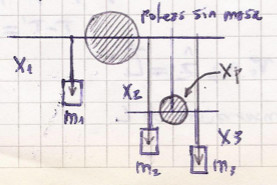
\includegraphics[scale=0.4]{images/fig_mc_dos_poleas.jpg}

Se tienen dos ecuaciones de vínculo
\[
	x_1 + x_p = \ell_1 \qquad \qquad (x_2 -x_p)+(x_3 -x_p) = \ell_2.
\]

El problema tiene cuatro coordenadas y dos ecuaciones de vínculo, lo cual nos deja dos grados de libertad.
La primer ecuación de vínculo permite liberarnos de $x_p$ y quedarnos en principio con los movimientos de
las tres masas. Entonces, ¿el principio de los trabajos virtuales? sería en este caso 
\[
	( m_1 \ddot{x}_1 - m_1 g )\delta x_1 + ( m_2 \ddot{x}_2 - m_2 g )\delta x_2 + ( m_3 \ddot{x}_3 - m_3 g )\delta x_3 = 0
\]
y luego podemos utilizar la segunda ecuación de vínculo, combinándola con la primera para llegar a 
\[
	x_2 + x_3 + 2x_1 = \text{ cte. }
\]
lo cual conduce a la relación 
\[
	\delta x_1 = -\frac{ \delta x_2 + \delta x_3 }{2}.
\]
Finalmente
\[
	( m_2 \ddot{x}_2 - m_2 g -\frac{m_1}{2} \ddot{x}_1 + \frac{m_1}{2} g ) \delta x_2 + 
	( m_3 \ddot{x}_3 - m_3 g -\frac{m_1}{2} \ddot{x}_1 + \frac{m_1}{2} g ) \delta x_3 = 0.
\]
\end{ejemplo}

\begin{notas}{Relación vínculos y desplazamientos:}
El hecho de que la fuerza de vínculo sea perpendicular a los desplazamientos puede
verse a partir de que la ecuación de vínculo en un sistema toma la forma
\notamargen{¿Y esta magia? Hay que aclarar realmente que sea así como se dice que es.}
\[
	f(\vb{x}_i) - K = 0 
\]
luego, derivando implícitamante cada ecuación y sumando (si se nos permite un pequeño
abuso de notación)
\[
	\sum_i^N \dpar{f}{\vb{x}_i} d\vb{x}_i = 0 
\]
pero esto no es otra cosa que
\[
	\nabla f \cdot \vb{\delta x} = 0
\]
donde debemos entender al gradiente y al vector $\vb{\delta x}$ como $N$ dimensionales.
\end{notas}


\subsection{Comentario vínculos}
\notamargen{Esto hay que consolidarlo todo. Volará.}
El trabajo de la fuerza de vínculos es nulo si el desplazamiento es virtual.
\[
	f(x_1,x_2,...,x_N,t) = 0
\]
\[
	\dpar{f}{x_1}\delta x_1 + ... +  \dpar{f}{x_N}\delta x_N = 0
\]
Como es un desplazamiento virtual, el tiempo $t$ está fijo (imagen fija = tiempo congelado)


% =================================================================================================
\section{Construcción del lagrangiano}
% =================================================================================================

Vamos a utilizar el principio de los trabajos virtuales para escribir las ecuaciones de la mecánica
de otra manera [¿?] sin preocuparnos por las fuerzas de vínculo, que en general pueden no ser 
conocidas o tener una naturaleza compleja.
\notamargen{Esta es la papa: las fuerzas de vínculo son difíciles de escribir si es esto posible 
del todo.}
Consideremos un sistema de $N$ partículas y $k$ ecuaciones de vínculo 
\begin{eqnarray*}
	& f_1(\vb{x}_1, \vb{x}_2,...,\vb{x}_n,t) = K_1  \\ 
	& ... ... ... \\
	& f_k(\vb{x}_1, \vb{x}_2,...,\vb{x}_n,t) = K_k 
\end{eqnarray*}
y por ende $3N-k$ grados de libertad (suponiendo que nos hallamos en 3 dimensiones).

Tenemos $N$ relaciones del tipo 
\be
	\vb{x}_i = \vb{x}_i(q_1,q_2,...,q_{3N-k},t)
	\label{x_part}
\ee
que significa que la posición de la partícula $i$-ésima depende en principio de las $3N-k$ coordenadas
generalizadas y del tiempo. Una variación de la misma tendrá la forma
\[
	\delta \vb{x}_i =  \sum_{j=1}^{3N-k} \left( \dpar{\vb{x}_i}{q_j} \right) \delta q_j + 
	\dpar{\vb{x}_i}{t}\delta t
\]
y suponiéndola un desplazamiento virtual el último término se anula puesto que $\delta t=0$ en ese
caso y entonces
\be
	\delta \vb{x}_i =  \sum_{j=1}^{3N-k} \left( \dpar{\vb{x}_i}{q_j} \right) \delta q_j.
	\label{delta_x_to_delta_q}
\ee

Por otro lado, del principio de los trabajos virtuales \eqref{principio_virtual_work} es
\[
	\sum_i^N \dot{\vb{p}}_i \cdot \delta \vb{x}_i - \sum_i^N  \vb{F}_i^a \cdot \delta \vb{x}_i = 0,
\]
donde $\vb{F}_i^a$ es la fuerza aplicada externa que no incluye las fuerzas de vínculo. El primer término 
se puede reescribir como
\[
	\dot{\vb{p}}_i \cdot \delta \vb{x}_i = m_i \dtot{\vb{v}_i}{t} \cdot \sum_{j=1}^{3N-k} 
	\left( \dpar{\vb{x}_i}{q_j} \right) \delta q_j,
\]
resultando
\be
	\sum_i^N m_i \dtot{\vb{v}_i}{t} \cdot \sum_{j=1}^{3N-k} \left( \dpar{\vb{x}_i}{q_j} \right)
	\delta q_j - \sum_i^N  \vb{F}_i^a \cdot \delta \vb{x}_i = 0
	\label{virtual_work_2}
\ee
Se ha pasado de una descripción en términos de $\delta \vb{x}_i$ ($3N$ variables) a otra en términos de $\delta q_j$
($3N-k$ coordenadas generalizadas).

La idea ahora es reescribir todo en términos más convenientes, para que aparezca un término multiplicado
a una variación arbitraria. De esta manera quedará una sumatoria de un sumando multiplicado por una
variación igualada a cero. No cabe otra posibilidad que el sumando sea nulo para cada índice de la suma.
\notamargen{Escrito muy mal este texto. La idea es clara, no obstante: hay que purificarla}

Consideremos en primer lugar la derivada total del producto siguiente
\[
	\frac{d}{dt}\left( m_i\vb{v}_i \cdot \dpar{\vb{x}_i}{q_j} \right) =
	m_i \dtot{\vb{v}_i}{t} \cdot \dpar{\vb{x}_i}{q_j} + m_i \vb{v}_i 
	\cdot \frac{d}{dt}\left(\dpar{\vb{x}_i}{q_j}\right),
\]
y en segundo lugar la velocidad de cada partícula, que proviene de la derivada total de cada ecuación 
\eqref{x_part} y resulta
% )Pero la diferencial del vector $\vb{x}_i$ es (notemos que no es una variación)
% \[
% 	d\vb{x}_i = \sum_{j=1}^{3N-k} \left( \dpar{\vb{x}_i}{q_j} \right) dq_j + \dpar{\vb{x}_i}{t} dt
% \]
% y entonces
\[
	\vb{v}_i = \dtot{\vb{x}_i}{t} = \sum_{j=1}^{3N-k} \left( \dpar{\vb{x}_i}{q_j} \right)
	\dot{q}_j + \dpar{\vb{x}_i}{t}.
\]

A partir de esta última es claro ver que la derivada de la velocidad de la partícula $i$-ésima respecto a la coordenada 
$l$-ésima es
\be
	\dpar{\vb{v}_i}{\dot{q}_l} = \dpar{\vb{x}_i}{q_l}.
	\label{relacion_derivadas}
\ee
\notamargen{Una manera menmotécnica de recordar esto es con el siguiente esquema:
\[
	\dpar{\vb{v}_i}{\dot{q}_l} = \frac{\partial \vb{x}_i/\partial t}{\partial q_l/\partial t} =
	\dpar{\vb{x}_i}{q_l}.
\]
}
La ecuación de la velocidad se puede derivar otra vez, con respecto a $q_l$, obteniéndose
\[
	\dpar{\vb{v}_i}{q_l} = \frac{\partial}{\partial q_l} \left( \dtot{\vb{x}_i}{t} \right) =
	\sum_{j=1}^{3N-k} \dparcru{\vb{x}_i}{q_j}{q_l} \dot{q}_j + 
	\dparcru{\vb{x}_i}{t}{q_l},
\]
y se puede ver que invirtiendo el orden de derivación, esto significa que 
\[
	\dpar{\vb{v}_i}{q_l} = \frac{d}{dt} \left( \dpar{\vb{x}_i}{q_l} \right).
\]

\notamargen{El hecho de que se pueda sacar fuera la derivada temporal y pasar adentro la derivada
con respecto a la coordenada generalizada $q$ puede verse haciendo la cuenta de manera explícita.}
% 
% \[
% 	\frac{d}{dt} \left( \dpar{\vb{x}_i}{q_l} \right) = 
% 	\frac{d}{dt} \left( \sum_{j=1}^{3N-k} \dparcru{\vb{x}_i}{q_j}{q_l} dq_j +
% 	\dparcru{\vb{x}_i}{t}{q_l} dt \right) 
% \]
% de tal manera que 
% \[
% 	\frac{d}{dt} \left( \dpar{\vb{x}_i}{q_l} \right) = \dpar{\vb{v}_i}{q_l}
% \]

Volviendo ahora a \eqref{virtual_work_2} y usando los resultados recientes tenemos
\[
	\sum_i^N \sum_{j=1}^{3N-k} 
	\left[ \frac{d}{dt} \left( m_i \vb{v}_i \dpar{\vb{x}_i}{q_j} \right) - 
	m_i \vb{v}_i \frac{d}{dt}\left( \dpar{\vb{x}_i}{q_j} \right) \right] \delta q_j
	- \sum_i^N  \vb{F}_i^a \cdot \delta \vb{x}_i = 0
\]
donde modificaremos el corchete expresando derivadas con respecto a la posición $\vb{x}$ en términos
de derivadas con respecto a la velocidad $\vb{v}$, de manera que 
\[
	\left[ \frac{d}{dt} \left( m_i \vb{v}_i \dpar{\vb{v}_i}{\dot{q}_j} \right) -
	m_i \vb{v}_i \dpar{\vb{v}_i}{q_j} \right]
\]
y usando el {\it trick} usual
\[
	\vb{v} \dpar{\vb{v}}{q} = \frac{1}{2} \dpar{ \vb{v}^2 }{q} 
\]
resulta
\[
	\left\{ 
	\frac{d}{dt} \left[ \frac{\partial}{\partial \dot{q}_j} \left( \frac{m_i}{2} \vb{v}_i^2 \right) \right] - 
	\frac{\partial}{\partial q_j} \left( \frac{m_i}{2} \vb{v}_i^2 \right) \right\}
\]

Es hora ya de introducir la sumatoria en $i$ hacia el interior del corchete, y la ecuación original es ahora 
\[
	\sum_{j=1}^{3N-k} \left\{ 
	\frac{d}{dt} \left[ \frac{\partial}{\partial \dot{q}_j}
	\left( \sum_i^N \frac{m_i}{2} \vb{v}_i^2 \right) \right] 
	- \frac{\partial}{\partial q_j} \left( \sum_i^N \frac{m_i}{2} \vb{v}_i^2 \right) \right\} \delta q_j
	- \sum_i^N  \vb{F}_i^a \cdot \delta \vb{x}_i = 0
\]
y dentro de los paréntesis ha aparecido la energía cinética $T$. La sumatoria en $j$ no era otra cosa que la suma 
de las derivadas de los momentos, y entonces
\[
	\sum_i^N \dot{\vb{p}}_i \cdot \delta \vb{x}_i =
	\sum_{j=1}^{3N-k} \left\{ \frac{d}{dt} \left[ \frac{\partial T}{\partial \dot{q}_j} \right] -
	\frac{\partial T}{\partial q_j} \right\} \delta q_j = \sum_i^N  \vb{F}_i^a \cdot \delta \vb{x}_i.
\]

Escribiendo la variación $\delta\vb{x}$ en términos de $\delta q$ a través de \eqref{delta_x_to_delta_q}
% \[
% 	\delta\vb{x}_i = \sum_{j=1}^{3N-k} \dpar{\vb{x}_i}{q_j}\delta q_j
% \]
se llega a 
\[
	\sum_{j=1}^{3N-k} \sum_i^N \left( \vb{F}_i^a \cdot \dpar{\vb{x}_i}{q_j} \right) \: \delta q_j =  
	\sum_{j=1}^{3N-k} Q_j \: \delta q_j
\]
siendo 
\[
	Q_j = \sum_i^N \left( \vb{F}_i^a \cdot \dpar{\vb{x}_i}{q_j} \right)
\]
la fuerza generalizada en el grado de libertad $j$. Entonces
\be
	\sum_{j=1}^{3N-k} \left\{ \frac{d}{dt}
	\left[ \frac{\partial T}{\partial \dot{q}_j} \right] - \frac{\partial T}{\partial q_j} - Q_j \right\} \delta q_j =  0
	\label{eq_el_0}
\ee
% y dado que las variaciones $\delta q_j$ son independientes se sigue que 

Si suponemos que las fuerzas son conservativas, provienen de un potencial, entonces 
\[
	\vb{F}_i^a = -\dpar{V(\{ \vb{x}_j \})}{\vb{x}_i}
\]
y expresando la fuerza $Q_j$ en términos del potencial $V$
\[
	Q_j = \sum_i^N \vb{F}_i^a \cdot \dpar{\vb{x}_i}{q_j} = 
	- \sum_i^N \dpar{V}{\vb{x}_i} \cdot \dpar{\vb{x}_i}{q_j} = -\dpar{V}{q_j},
\]
el cual, insertado en la ecuación \eqref{eq_el_0}, conduce a
\[
	\sum_{j=1}^{3N-k} \left\{ \frac{d}{dt}
	\left[ \frac{\partial T}{\partial \dot{q}_j} \right] - \frac{\partial}{\partial q_j} \left( T - V \right) \right\} \delta q_j =  0.
\]
% \[
% 	Q_j \: \delta q_j = -\dpar{V}{q_j} \: \delta q_j
% \]
% y como $V=V(\vb{x}_1,...,\vb{x}_n)$ se tiene 
% \[
% 	V = \sum_i^N  \dpar{V}{r_i} \delta \vb{x}_i = \dpar{V}{\vb{x}_i} \cdot \dpar{\vb{x}_i}{q_j} \delta q_j =
% \]
% pero 
% \[
% 	Q_j = - \dpar{V}{q_j}
% \]
% y entonces 
% \[
% 	\sum_{j=1}^{3N-k} \left\{ 
% 	\frac{d}{dt} \left( \dpar{T}{\dot{q}_j} \right) - \frac{\partial}{\partial q_j}
% 	\left( T - V \right) \right\} \delta q_j =  0.
% \]
Dado que $ V = V(\vb{x}_1,...,\vb{x}_N) = V( \{ q_j \} )$ (no depende de las velocidades generalizadas $ \dot{q}_j $) se puede escribir 
\[
	\sum_{j=1}^{3N-k} \left\{ \frac{d}{dt}
	\left[ \frac{\partial}{\partial \dot{q}_j} \left( T - V \right) \right] - 
	\frac{\partial}{\partial q_j} \left( T - V \right) \right\} \delta q_j =  0.
\]
y definiendo al lagrangiano\index{Lagrangiano} $\Lag$ como 
\[
	\Lag \equiv T - V
\]
se arriba a
\[
	\sum_{j=1}^{3N-k} \left[
	\frac{d}{dt} \left( \dpar{\Lag}{\dot{q}_j} \right) -  \dpar{\Lag}{q_j} \right] \delta q_j =  0.
\]
Nótese que $\Lag = \Lag( q_1,...,q_{3N-k}, \dot{q}_1, ..., \dot{q}_{3N-k}, t ) $, es decir que es función 
del conjunto $(\{ q_j \}, \{ \dot{q}_j \}, t)$. De esta manera las ecuaciones resultantes serán, a lo sumo,
ecuaciones diferenciales para $q_j(t)$ de orden dos.

Si existieran fuerzas aplicadas que no provienen de un potencial (no conservativas) entonces
\[
	Q_j + Q_j^{NC} = -\dpar{V}{q_j} + Q_j^{NC},
\]
y las ecuaciones adquieren un término extra 
\[
	\sum_{j=1}^{3N-k} \left[
	\frac{d}{dt} \left( \dpar{\Lag}{\dot{q}_j} \right) - \dpar{\Lag}{q_j} - Q_j^{NC} \right] \delta q_j = 0.
\]

Como esto vale para todo grado de libertad $j$, puesto que las variaciones son independientes, llegamos a
\[
	\frac{d}{dt} \left( \dpar{\Lag}{\dot{q}_j} \right) -  \dpar{\Lag}{q_j} = Q_j^{NC}
\]
que son las ecuaciones de Euler-Lagrange con presencia de fuerzas no conservativas. 
Este es el resultado más importante del capítulo.
\notamargen{No sé si es la primera vez que aparecen. De serlo habría que remarcarlo como es debido, tal vez
recuadrar}

Se tienen así una formulación para los problemas mecánicos en términos de ecuaciones diferenciales para los
grados de libertad $q_j$ que prescinden del conocimiento de las fuerzas de vínculo.

\subsection{Algunos ejemplos del lagrangiano}

% ~~~~~~~~~~~~~~~~~~~~~~~~~~~~~~~~~~~~~~~~~~~~~~~~~~~~~~~~~~~~~~~~~~~~~~

\begin{ejemplo}{\bfseries Bloques deslizantes}

Teníamos el vínculo 
\[
	-2x_1 + x_2 = \text{ cte. }
\]
Luego,
\[
	T = \frac 1 2 m_1 \dot{x}_1^2 + \frac 1 2 m_2 \dot{x}_2^2 \qquad \qquad V = -m_2 g x_2
\]
y tomando $x_2$ como independiente llego a
\[
	T-V = \frac{1}{2}\left( \frac{m_1}{4} + m_2 \right) \dot{x}_2^2 + m_2gx_2.
\]
Luego, las ecuaciones de E-L serán
\[
	\dtot{}{t}\left( \dpar{\Lag}{\dot{x}_2} \right) - \dpar{\Lag}{x_2} =
	\left( \frac{m_1}{4} + m_2 \right) \ddot{x}_2 - m_2 g = 0
\]
que conduce a 
\[
	\ddot{x}_2 = \frac{m_2 g}{\frac{m_1}{4} + m_2 },
\]
que es a lo que se tenía que llegar.
\end{ejemplo}

\begin{ejemplo}{\bfseries Péndulo}

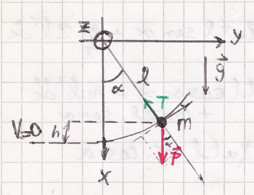
\includegraphics[scale=0.35]{images/fig_mc_pendulo_lag.jpg}

Las ecuaciones son 
\[
	m\ell \dot{\alpha}^2 = - T + m g \cos \alpha \qquad 
	m\ell \ddot{\alpha} = - m g \sin \alpha
\]
y se podría resolver desde aquí nomás. Pero escribamos el lagrangiano
\[
	\Lag = T-V = \frac 1 2 m \ell^2 \dot{\alpha}^2 - mg\ell(1-\cos \alpha)
\]
Sus ecuaciones de E-L son
\[
	m \ell \ddot{\alpha} + mg\ell \sin \alpha = 0
\]
que es la ecuación del péndulo $\ddot{\alpha} = -g/\ell \sin \alpha$.

\end{ejemplo}

\begin{ejemplo}{\bfseries Aro acelerado }

\notamargen{Falta ilustración del aro y sistema coordenado.}
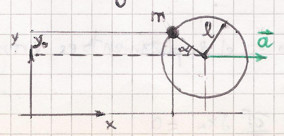
\includegraphics[scale=0.35]{images/fig_mc_aro_acelerado_lag.jpg}

Supongamos un aro horizontal en una mesa sin rozamiento. Tiene un único grado de libertad.

El vínculo es
\[
	(x - \nicefrac{1}{2} \: at^2)^2 + (y-y_0 )^2 = \ell^2
\]
y las posiciones instantáneas de la masa $ m $
\[
	x = \frac{1}{2}at^2 - \ell \cos(\vp) \qquad  y = y_0 + \ell \sin(\vp)
\]

Es conveniente utilizar el ángulo $\vp$ como coordenada generalizada. Pero $\vp$ está solidaria al aro.
Eso no es un problema siempre que el $\Lag$ esté medido en un sistema inercial.

En este caso no hay potencial pero como $\vp$ es una coordenada vista en un sistema no inercial, aparecerán
las fuerzas ficticias asociadas al movimiento.
Serán
\[
	\dot{x} = at + \ell \sin(\vp) \dot{\vp} \qquad \dot{y} = \ell \cos(\vp) \dot{\vp}
\]
\notamargen{La $T$ del $\Lag$ es la vistda desde un sistema INERCIAL siempre; en todo caso luego aparecen
las fuerzas ficticias necesarias. ESTO HAY QUE ESTUDIARLO Y ENTENDERLO.
}
y luego 
\[
	\Lag = T = \frac{1}{2} m (\dot{x}^2 + \dot{y}^2 ) = \frac{1}{2} m
	(a^2 t^2 + 2at\ell\sin(\vp)\dot{\vp}+\ell^2\dot{\vp}^2)
\]

Las ecuaciones de Euler-Lagrange serán 
\[
	\dtot{}{t}\left( \dpar{\Lag}{\dot{\vp}}\right) - \dpar{\Lag}{\vp} = 
	m \ell^2 \ddot{\vp} + ma\ell \sin(\vp) = 0
\]
lo cual resulta en la ecuación de movimiento
\notamargen{El lagrangiano se dedujo de las ecuaciones de Newton, entonces debemos calcular $T,V$ de un sistema
inercial. Acá no se entiende si lo que se hace en la carpeta está bien o no, en el sentido de que parece que al
usar una coordenada que no es inercial estamos calculando T no inercial.? }
\[
	\ddot{\vp} = - \frac{a}{\ell} \sin(\vp) 
\]
que es una ecuación que da oscilaciones, como la de un péndulo. Estas oscilaciones están causadas, claramente,
por la aceleración $a$.

En este ejemplo se ve que se calcula la energía cinética $T$ en un sistema inercial; no obstante, este valor está
expresado en términos de una coordenada que no es inercial (es solidaria al aro). Aparecen entonces las fuerzas 
inerciales que tienen que aparecer y punto.
\end{ejemplo}
% ~~~~~~~~~~~~~~~~~~~~~~~~~~~~~~~~~~~~~~~~~~~~~~~~~~~~~~~~~~~~~~~~~~~~~~

\begin{ejemplo}{\bf Problema 5 --para vínculos--}

Este problema es de vínculos y trabajos virtuales. Habría que reubicarlo.

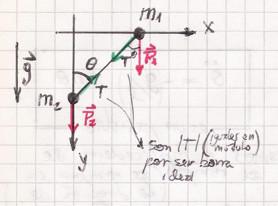
\includegraphics[scale=0.35]{images/fig_mc_oscilador_barra.jpg}

Se tienen dos masas $m_1$ y $m_2$ de manera que en principio se tendrían seis coordenadas; no obstante como el movimiento
es en un plano (se puede tomar el $z=0$ como tal) y las masas están restringidas a moverse a lo largo del eje que las
engarza se tiene, adoptando el esquema de la figura,
\[
	z_1 = z_2 = 0 \qquad \qquad x_2 = y_1 = 0
\]
es decir cuatro ecuaciones de vínculo a la cual le sumamos una quinta
\be
	x_1^2 + y_2^2 = \ell^2
	\label{vinculo_problema_5}
\ee
de manera que resulta un problema para un único grado de libertad. Obviando los subíndices que no son necesarios, y diferenciando
implícitamente la ecuación \eqref{vinculo_problema_5} se obtiene 
\[
	x dx + y dy = 0 
\]
Utilizando el ángulo $\theta$ y parametrizando las variables implicadas en \eqref{vinculo_problema_5} de acuerdo con 
\[
	x = \ell \sin \theta \qquad y = \ell \cos \theta
\]
vemos que es una buena coordenada porque verifica el vínculo de manera natural.

Planteando las ecuaciones 
\[
	( T \sin \theta - m_1 \ddot{x} ) \delta x + ( m_2 g - T \cos \theta - m_2 \ddot{y} ) \delta y = 0
\]
\be
	x \delta x = -y \delta y
	\label{relacion_deltas}
\ee
pero usando la última, se tiene
\[
	-\frac{x}{\ell}T\delta x - \frac{y}{\ell}T\delta y = 0 
\]
de manera que desaparece la tensión. Entonces
\[
	m_2 \ddot{x} \delta x = m_2 (g - \ddot{y}) \delta y
\]
que es una ecuación de Lagrange de primera especie. Usando otra vez \eqref{relacion_deltas}
\[
	- m_1 \ddot{x} \frac y x = m_2 (g - \ddot{y})
\]
y entonces ahora habría que convertir a expresar todo en términos de $\theta$. Derivando las expresiones de $x,y$ en términos
del ángulo $\theta$ resulta que 
\[
	-m_1 \ell ( \ddot{\theta} \cos \theta - \dot{\theta}^2 \sin \theta ) \frac{\cos \theta}{\sin \theta}  = 
	m_2 ( g + \ell \ddot{\theta} \sin \theta + \ell \dot{\theta} \cos \theta )
\]
\[
	\ddot{ \theta } \ell ( m_2 \sin \theta + m_1 \frac{\cos^2 \theta}{\sin \theta} ) + 
	\dot{\theta}^2 \ell (m_2 \sin \theta - m_1 \cos \theta ) + m_2 g = 0
\]
Si $ m_1 = m_2 $ entonces
\[
	\ddot{ \theta } \ell \frac{m}{\sin \theta} + m  g = 0 
\]
\[
	\ddot{ \theta } = -\frac{ g }{ \ell } \sin \theta,
\]
y vemos que es un péndulo.

Ahora se quisiera calcular la tensión $T$. Se utilizarán multiplicadores de Lagrange. Sea que los vínculos se rompen (se rompen, por supuesto, en la 
dirección de las fuerzas de vínculos). Supongamos que existe $y_1$ (hay desplazamiento en la coordenada $y_1$) entonces existirá $\lambda$ tal que 
$\lambda  \delta y_1 \neq 0$
\[
	\delta y_1 ( m_1 \ddot{y}_1 - \lambda - m_1 g ) \qquad \lambda = m_1 g
\]
pero la ecuación en (1) (página anterior) debe seguir valiendo.
\[
	\lambda_T + x \delta x + \lambda_T y \delta y 
\]
\[
	( m_1 \ddot{x} + \lambda_T x ) \dx + ( m_2 (g - \ddot{y} ) + \lambda_T + y ) \dy = 0
\]
lo cual vale si $\lambda_T = - \frac T \ell $.
Y se ve que el multiplicador de Lagrange es la tensión (vínculo) -- la fuerza asociada a que se cumpla el vínculo --.
Tengo un multiplicador por cada vínculo. Si hay $n$ vínculos y quiero un vínculo uso un solo multiplicador.
Pero ahora $\dx$ y $\dy$ son independientes, entonces deben anularse por separado los dos miembros de la ecuación de Newton.
\[
	m_1 \ddot{x} + \lambda_T x  \qquad \qquad m_ 2(g -\ddot{y}) + \lambda_T y
\]
\[
	\lambda_T = - \frac{m_1 \ddot{x}}{x} 
\]
\[
	\lambda_T = -\frac{ m_1 ( \ddot{ \theta } \cos \theta - \dot{\theta}^2 \sin \theta ) }{\sin \theta} =
	m_1 (\frac g \ell \cos \theta - \dot{\theta}^2 )
\]
\end{ejemplo}



% =================================================================================================
\section{Invariancia del lagrangiano ante adición de una derivada total}
% =================================================================================================

En los ejemplos del péndulo y del aro acelerado [CITAR], la resolución del sistema a través de las ecuaciones de 
Euler-Lagrange condujo a las mismas ecuaciones de movimiento (lo que signfica que, para iguales condiciones iniciales, 
la física del sistema es la misma) pero se partió de dos lagrangianos diferentes
\[
	\Lag = \frac 1 2 m \ell^2 \dot{\alpha}^2 + m g \ell \cos \alpha \qquad
	\Lag'= \frac 1 2 m \left( \ell^2 \ddot{\alpha} + 2 \ell g t \sin \alpha \: \dot{\alpha} + g^2 t^2 \right)
\]
\notamargen{La aceleración del aro era $a$ pero escribimos $g$ para enfatizar que tienen la misma forma.}
que llevaban a
\[
	\ell \ddot{\alpha} + g \sin \alpha = 0. 
\]
Es decir, que desde el punto de vista del movimiento del sistema, los dos lagrangianos son equivalentes.
Pero notemos que el término central en $\Lag'$ aparece vinculado a 
\[
	\dtot{}{t}\left( m l g t \cos \alpha \right) = -m \ell g t \dot{\alpha} \sin \alpha + m l g \cos \alpha,
\]
de manera que 
\[
	\Lag'= \frac 1 2 m \ell^2 \dot{\alpha}^2 + m l g \cos \alpha -
	\dtot{}{t}\left( m l g t \cos \alpha \right) + \frac 1 2 g^2 t^2
\]
\[
	\Lag'= \frac 1 2 m \ell^2 \dot{\alpha}^2 + m l g \cos \alpha - 
	\dtot{}{t}\left( m l g t \cos \alpha - \frac 1 6 g^2 t^3 \right)
\]
o bien 
\[
	\Lag' = \Lag + \dtot{}{t}(F(\alpha,t)).
\]

Entonces, parece que existe alguna relación entre dos lagrangianos que conducen a iguales ecuaciones de movimiento.

En el ejemplo visto del sistema mecánico del aro acelerado parece que existía alguna relación entre dos 
lagrangianos que conducían a iguales ecuaciones de movimiento. Veamos ahora el origen de esa relación.
\notamargen{Link con el ejemplo del aro acelerado!!}

Dado un lagrangiano $\Lag = \Lag(\dot{q}_i,q_i,t)$ nos construimos otro $\Lag'$ sumándole al anterior la 
derivada total de una función arbitraria de las coordenadas y del tiempo $F=F(q_i,t)$, de modo que
\[
	\Lag'(\dot{q}_i,q_i,t) = \Lag(\dot{q}_i,q_i,t)+ \dtot{F}{t}(q_i,t) .
\]

Las ecuaciones de Euler-Lagrange 
\[
	\frac{d}{dt}\left(\dpar{\Lag'}{\dot{q}_j}\right) - \dpar{\Lag'}{q_j} = 0
\]
para este nuevo lagrangiano resultan en
\begin{multline}
 	\qquad \frac{d}{dt}\left(\dpar{\Lag'}{\dot{q}_j}\right) - \dpar{\Lag'}{q_j} =
 	\dtot{}{t}\left(\dpar{\Lag}{\dot{q}_j}\right) - \dpar{\Lag}{q_j} + \\
 	\dtot{}{t}\left(\dpar{}{\dot{q}_j}\left[ \dtot{F}{t} \right]\right) 
	- \dpar{}{q_j}\left[ \dtot{F}{t}\right] = 0 \qquad \label{ecEL_lag_suma}	
\end{multline}
% \[
% 	\dtot{}{t}\left(\dpar{\Lag}{\dot{q}_j} + \dpar{}{\dot{q}_j}\left(\dtot{F}{t}\right)\right) -
% 	\dpar{\Lag}{q_j} - \dpar{}{q_j}\left( \dtot{F}{t}\right) = 0 
% \]
donde aparecen las ecuaciones correspondientes al lagrangiano $\Lag$ más los dos términos del 
renglón inferior.
Veremos que estos se cancelan exactamente por un argumento similar al encontrado en la ecuación
\eqref{relacion_derivadas} en la sección anterior.
% \[
% 	\dtot{}{t}\left(\dpar{\Lag}{\dot{q}_j}\right) - \dpar{\Lag}{q_j} + 
% 	\dtot{}{t}\left(\dpar{}{\dot{q}_j}\left(\dtot{F}{t}\right)\right) 
% 	- \dpar{}{q_j}\left( \dtot{F}{t}\right) = 0 
% \]

Para ello es necesario expresar la derivada total de $F$,
\[
	\dtot{F}{t} = \sum_i^{3N-k} \left( \dpar{F}{q_i} \right) \dot{q}_i + \dpar{F}{t}
\]
y ver que
\[
	\dpar{}{\dot{q}_j}\left[ \dtot{F}{t}\right] = \dpar{F}{q_j} \qquad\qquad
	\dpar{}{q_j}\left[ \dtot{F}{t}\right] = \dpar[2]{F}{q_j} \dot{q}_j + \dparcru{F}{t}{q_j} 
\]

Usando explícitamente estos resultados en los términos extra de \eqref{ecEL_lag_suma}, se llega 
a que 
\begin{multline*}
 	\dtot{}{t}\left(\dpar{}{\dot{q}_j}\left[ \dtot{F}{t} \right]\right) 
	- \dpar{}{q_j}\left[ \dtot{F}{t}\right] =
	\dtot{}{t}\left( \dpar{F}{q_j} \right) - \dpar{}{q_j}\left( \dtot{F}{t}\right) = \\
	\left\{ \dpar[2]{F}{q_j} \: \dot{q}_j + \dparcru{F}{q_j}{t} \right\}%- \dpar{}{q_j}\left( \dtot{F}{t}\right)
	- \left\{ \dpar[2]{F}{q_j} \dot{q}_j + \dparcru{F}{t}{q_j} \right\} =
	\dparcru{F}{q_j}{t} - \dparcru{F}{t}{q_j} = 0
\end{multline*}
% \[
% 	\dtot{}{t}\left( \dpar{}{\dot{q}_j}\left(\dtot{F}{t}\right)\right) - 
% 	\dpar{}{q_j}\left( \dtot{F}{t}\right) = \dtot{}{t}\left( \dpar{F}{q_j} \right) - 
% 	\dpar{}{q_j}\left( \dtot{F}{t}\right)
% \]
% \[
% 	\dtot{}{t}\left( \dpar{F}{q_j} \right) - \dpar{}{q_j}\left( \dtot{F}{t}\right) =
% 	\dpar[2]{F}{q_j} \dot{q}_j + \dparcru{F}{q_j}{t} - \dpar{}{q_j}\left( \dtot{F}{t}\right)
% \]
donde la obtención del cero responde a que hemos aceptado que las derivadas cruzadas de $F$ son idénticas.
Para ello basta con admitir que $F$ sea de clase $C^2$ (derivadas segundas continuas).

Finalmente hemos comprobado que las ecuaciones de Euler Lagrange no se modifican si añadimos al lagrangiano la 
derivada total respecto del tiempo de una función de $(q_i,t)$.
O sea que podríamos construir infinitos lagrangianos diferentes por el añadido de una derivada total y todos
ellos llevan a las mismas ecuaciones de movimiento.

\begin{ejemplo}{\bf Lagrangiano en funcionamiento}

Dos masas $m_1, m_2$ conectadas mediantes barras rígidas de masa despreciable según indica la figura que se mueven en 
un plano.

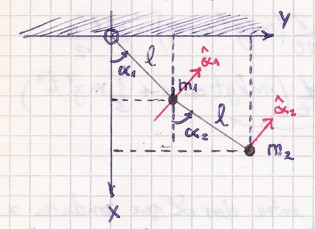
\includegraphics[scale=0.35]{images/fig_mc_clasica_pendulo_doble.jpg}

En principio este problema tiene cuatro coordenadas $x_1,x_2,y_1,y_2$ pero las barras determinan dos ecuaciones de 
vínculo
\[
	x_1^2 + y_1^2 = \ell  \qquad \qquad (x_2-x_1)^2 + (y_2-y_1)^2 = \ell^2
\]
de modo que es un sistema con dos grados de libertad.

\notamargen{Este ejemplo es interesante porque considera unos versores movibles. Habría que continuarlo y ver qué se 
hizo en la carpeta.} 

Para escribir el lagrangiano notemos que 
\[
	T = T_1 + T_2 = \frac 1 2 m_1 ( \dot{x}_1^2 + \dot{y}_1^2 ) + \frac 1 2 m_2 ( \dot{x}_2^2 + \dot{y}_2^2 ) 
\]
\[
	V = -m_1 g x_1 - m_2 g x_2
\]

Y en términos de los ángulos $\alpha_1$, $\alpha_2$ se tiene 
\[
	x_1 = \ell \cos \alpha_1 \qquad y_1 = \ell \sin \alpha_1 
\]
\[
	x_2 = \ell \cos \alpha_2 + \ell \cos \alpha_1 \qquad y_2 = \ell \sin \alpha_1 + \ell \sin \alpha_2
\]
pero antes de hacer toda el álgebra, notemos que $( \dot{x}_1^2 + \dot{y}_1^2 ) = |\vb{v}_1| $ está siempre en la 
dirección del vector $\hat{\alpha}_1$ y no puede tener componente perpendicular. Considerando solamente esa componente, 
sería
\[
	\vb{v}_1 = \ell \: \dot{\alpha}_1 \hat{\alpha}_1 \qquad \text{ con } \qquad v_1^2 = \ell^2 \: \dot{\alpha}_1^2
\]
y correspondientemente
\[
	\vb{v}_2 = \ell \: \dot{\alpha}_1 \hat{\alpha}_1 + \ell \: \dot{\alpha}_2 \hat{\alpha}_2
\]
\[
	v_2^2 = \ell^2 \: \dot{\alpha}_1^2 + \ell^2 \: \dot{\alpha}_2^2 + 2 \dot{\alpha}_1 \dot{\alpha}_2 \ell^2
	\cos ( \alpha_2 - \alpha_1 ).
\]
\end{ejemplo}


% =================================================================================================
\section{Momentos conjugados y coordenadas cíclicas}\index{Momentos conjugados} \index{Coordenadas cíclicas}
% =================================================================================================

Dado un lagrangiano $\Lag = \Lag( q_i,\dot{q}_i, t )$ se define el momento canónicamente conjugado a $q_j$
como 
\be
	p_j \equiv \dpar{\Lag}{\dot{q}_j},
	\label{mom_canon_conj}
\ee
y entonces 
\[
	\dot{p}_j = \frac{d}{dt}\left( \dpar{\Lag}{\dot{q}_j} \right) \equiv Q_j,
\]
que es la fuerza generalizada en el grado de libertad $j$.

Sea ahora un lagrangiano que no depende explícitamente de la coordenada $k$, es decir 
\[
	\Lag = \Lag( q_1,...,q_{k-1},q_{k+1},...,q_n,\dot{q}_1,...\dot{q}_n, t ),
\]
entonces será
\[
	\dpar{\Lag}{q_k}= 0 
\]
y como consecuencia las ecuaciones de Euler-Lagrange en la coordenada $k$-ésima resultan 
\[
	\dtot{}{t}\left( \dpar{\Lag}{\dot{q}_k} \right) = \dot{ p }_k = Q_k = 0 
% 	\quad \rightarrow \;\dot{p}_k = 0 \quad \rightarrow \; p_k = cte.
\]
de manera que no existe fuerza generalizada en el grado de libertad $k$ y como es $\dot{p}_k = 0$, se conserva 
el momento $p_k$ canónicamente conjugado a $q_k$.
En estos casos se dice que la coordenada $q_k$ que no aparece en el lagrangiano, es una coordenada
cíclica.

\begin{ejemplo}{\bf Potencial central en un plano}

Sea un potencial central $ V(r) $ en el plano. El lagrangiano de una partícula de masa $m$ sometida al mismo,
y en las convenientes coordenadas polares $(r,\vp)$ es
\[
	\Lag = \frac{1}{2} m ( \:\dot{r}^2 + r^2 \dot{\vp}^2 ) - V(r).
\]
Luego, las ecuaciones de Euler-Lagrange serán, en $r$,
\[
	\dtot{}{t}\left( \dpar{\Lag}{\dot{r}}\right) - \dpar{\Lag}{r} =
	m\ddot{r} - m\dot{\vp}^2r + \dtot{V}{r} = 0
\]
y en $\vp$
\[
	\dtot{}{t}\left( \dpar{\Lag}{\dot{\vp}}\right) = mr^2\ddot{\vp} = 0.
\]
En esta última debemos notar que $\partial \Lag / \partial \vp = 0 $ y esto significa que $\vp$ es cíclica.
Entonces se conserva el momento canónicamente conjugado a $\vp$ puesto que verifica 
\[
	\dot{p}_\vp = mr^2\ddot{\vp} = 0
\]
lo cual lleva a que $ m r^2\dot{\vp} $ es una constante para este sistema. La moraleja es que la existencia de una 
coordenada cíclica permite ahorrarnos una integración.
Esto, por supuesto, para este problema no es otra cosa que la conservación del momento angular [?].

\end{ejemplo}

% =================================================================================================
\section{Momentos canónicamente conjugados y traslaciones rígidas}
% =================================================================================================

Consideremos un sistema de partículas que sufre una traslación rígida infinitesimal.
Esta traslación se lleva a cabo a través de un desplazamiento en la coordenada $ q $ y de magnitud 
$\delta q$ en la dirección dada por el versor $ \hat{n} $.
% Esta coordenada justamente tiene esa propiedad: una variación de ella representa una 
% traslación rígida.
% ESTE COMENTARIO, que estaba en la carpeta, ahora queda un poco desplazado por la sentencia más
% correcta con respecto a la dirección \hat{n}. Supongo que lo importante es la dirección que en
% el caso de cartesianas la da la misma q pero que en el caso de versores que varían su dirección
% curvilíneos, debe especificarse.

En efecto, para el sistema de $ N $ partículas, la traslación rígida implica
\[
	q \longrightarrow q + \delta q \qquad 
	\vb{x}_i \longrightarrow \vb{x}_i + \delta q \; \hat{n}
\]
La Figura \ref{traslacion_rigida} representa la situación.

Luego, suponiendo una energía cinética de tipo $T_2$, el momento canónicamente conjugado $ p $ (en 
la coordenada $q$ --cuyo subíndice omitimos--) es
\notamargen{[¿se sabe esto a esta altura?]}
\[
	p = \dpar{T}{\dot{q}} = \frac{1}{2} \sum_i^N m_i \left( \dpar{\vb{v}_i^2}{\dot{q}}\right) =
	\sum_i^N m_i \vb{v}_i \cdot \dpar{\vb{v}_i}{\dot{q}} 
\]
\notamargen{Hablar de vectores al cuadrado.\\}
\notamargen{\\ Nota de cómo se manipula: uso $dv^2_i = 2 v_i dv_i$ y}

La {\it forma} de la traslación rígida implica que 
\[
	\dpar{\vb{v}_i}{\dot{q}} = \dpar{\vb{x}_i}{q} = 
	\lim_{\delta q \to 0} \frac{\vb{x}_i + \delta q \:\hat{n} -\vb{x}_i}{\delta q} = \hat{n}.
\]
\notamargen{Recodemos que $ \vb{v}_i = \dot{q}_j\dpar{\vb{x}_i}{q_j} - \dpar{\vb{x}_i}{t} $ }
de modo que 
\[
	p = \sum_i^N m_i \vb{v}_i \cdot \hat{n} = \left( \sum_i^N m_i \vb{v}_i \right) \cdot \hat{n} 
	= \vb{P} \cdot \hat{n} = P_{\hat{n}}
\]

\begin{figure}[htb]
	\begin{center}
	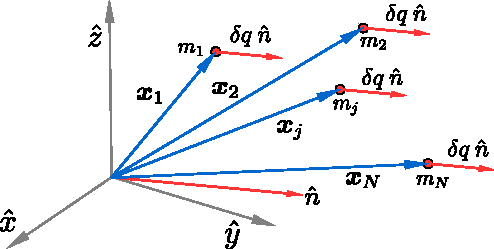
\includegraphics[width=0.6\textwidth]{images/fig_mc_tras_rig.pdf}	 
	\end{center}
	\caption{}
	\label{traslacion_rigida}
\end{figure} 

Hemos arribado al resultado de que el momento canónicamente conjugado correspondiente a la coordenada
generalizada asociada a la traslación rígida es la proyección del momento total en la dirección de ésta.

Para el ejemplo trivial de la partícula libre, $T = 1/2 \; m (\dot{x}^2+ \dot{y}^2+\dot{z}^2)$, se
tiene $ p_x = m v_x $ si la traslación es en la dirección $ \hat{x} $.
\notamargen{Este ejemplo suma algo?}

Para las fuerzas generalizadas, equivalentemente se tiene 
\[
	Q = \sum_i^N \vb{F}^a_i \cdot \dpar{\vb{x}_i}{q} =
	\left( \sum_i^N \vb{F}^a_i \right) \cdot \hat{n} = \vb{F}\cdot \hat{n},
\]
la fuerza generalizada es la proyección de las fuerzas aplicadas en la dirección dada por $ \hat{n} $.

\notamargen{Revisar porque esto no estaba tan claro. Supongo que la idea es ver que aún con presencia
de $T_1$ esto sigue valiendo}
La ecuación para la fuerza generalizada $Q_j$ era
\[
	Q_j = \frac{d}{dt}\left( \dpar{T}{\dot{q}_j} \right) - \dpar{T}{q_j}.
\]
Aún en el caso de que $T$ dependa de $q_j$ la traslación rígida implica que 
$ \partial{T}/\partial{q_j} = 0 $ 
porque es sumar un vector constante a la posición, luego $ d\vb{x}_i/dt = d(\vb{x}_i + \vb{a}) /dt$
para todo \vb{a} constante. Entonces, para la coordenada q asociada a la traslación en $\hat{n}$
se tiene 
% \[
% 	Q_j = \frac{d}{dt}\left( \dpar{T}{\dot{q}_j} \right)
% \]
% y en el caso de la traslación con dirección $\hat{n}$,
\[
	Q = \frac{d}{dt}\left( \dpar{T}{\dot{q}} \right) = \dtot{P_{\hat{n}}}{t},
\]
de tal manera que si en $\hat{n}$ no hay fuerza $Q$ tendremos $ d P_{\hat{n}}/dt = 0 $, es decir 
$ P_{\hat{n}} $ conservado.

\notamargen{Acá la cosa es que la traslación es una cosa que sufre el sistema pero no es dinámica.
Es una construcción nuestra, como un cambio de sistema de referencia.}

% pero el segundo término del lado izquierdo $\partial T/\partial q_j = 0$ puesto que la $T$ no se ve
% afectada por cambiar trasladando rígidamente el sistema.
% \[
% 	\frac{d}{dt}(\vb{p}\cdot \hat{n}) = \vb{F}\cdot \hat{n},
% \]
% y esto significa que el $p_j$ se conserva si no hay fuerza en $\hat{j}$.

% =================================================================================================
\section{Momentos canónicamente conjugados y rotaciones rígidas}
% =================================================================================================

Ahora consideraremos un sistema de partículas que sufre una rotación rígida infinitesimal.
Esta se materializa a través de un desplazamiento angular en la coordenada $ q $ de magnitud $\delta q$.
La dirección y sentido, para cada posición $ \vb{x}_i $ vienen dadas por el producto vectorial 
$ \hat{n} \times \vb{x}_i$.

\notamargen{Esta coordenada $q$ es especial en el sentido en que representa una rotación.}
Para un sistema de $ N $ partículas, la rotación rígida implica
\[
	q \longrightarrow q + \delta q |\vb{x}| \sin \alpha_i \qquad
	\vb{x}_i \longrightarrow \vb{x}_i + \delta q \; \hat{n} \times \vb{x}_i
\]
La Figura \ref{rotacion_rigida} representa la situación, donde por razones de claridad se muestran
solamente dos partículas.

\begin{figure}[htb]
	\begin{center}
	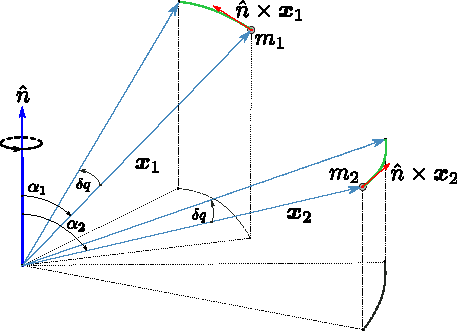
\includegraphics[width=0.6\textwidth]{images/fig_mc_rot_rig.pdf}	 
	\end{center}
	\caption{}
	\label{rotacion_rigida}
\end{figure} 
% Ahora es el turno de la rotación rígida. Sea coordenada que representa rotación rígida,
% \[
% 	\vb{r}_i \longrightarrow \vb{r}_i + \delta q (\hat{n} \times \vb{r}_i)
% \]
El momento canónicamente conjugado en la coordenada angular $q$ será
\[
	p = \dpar{T}{\dot{q}} = 
	\sum_i^N m_i \vb{v}_i \cdot \dpar{\vb{v}_i}{\dot{q}} =
	\sum_i^N m_i \vb{v}_i \cdot \hat{n} \times \vb{x}_i = 
	\sum_i^N m_i \vb{v}_i \cdot ( \hat{n} \times \vb{x}_i )
\]
donde hemos utilizado el hecho de que 
\[
	\dpar{\vb{v}_i}{\dot{q}} = \dpar{\vb{x}_i}{q} = 
	\lim_{\delta q \to 0} \frac{ \vb{x}_i +\delta q (\hat{n} \times \vb{x}_i)- 
	\vb{r}_i}{\delta q} = \hat{n} \times \vb{x}_i. 
\]

El sumando se puede reescribir (usando $\vb{A}\cdot(\vb{B}\times\vb{C}) = 
\vb{B}\cdot(\vb{C}\times\vb{A})$) para que aparezca explícitamente la forma buscada,
\[
	p = \sum_i^N m_i \vb{v}_i \cdot ( \hat{n} \times \vb{x}_i ) =
	\sum_i^N \hat{n} \cdot ( \vb{x}_i \times m_i \vb{v}_i  ) =
	\sum_i^N \hat{n} \cdot \vb{l}_i = \hat{n} \cdot \sum_i^N \vb{l}_i =
	\hat{n} \cdot \vb{L}
\]
que significa
\[
	p = \hat{n} \cdot \vb{L} = L_{\hat{n}},
\]
el momento canónicamente conjugado en la dirección $\hat{n}$ es el momento angular total
del sistema proyectado en esa dirección.
% \[
% 	|\delta q(\hat{n} \times \vb{r}_i)| = \delta q r_i \sin (\alpha)
% \]
% El momento canónicamente conjugado en la dirección $\hat{n}$ es el $\vb{L}$ proyectado en esa dirección.
% \[
% 	\frac{d}{dt}(\hat{n}\cdot\vb{L}) = \hat{n}\cdot\vb{\tau}
% \]
% y el $p_j$ se conserva si no hay torque.
La fuerza generalizada será
\[
	Q = \sum_i^N \vb{F}^a_i \cdot \dpar{\vb{x}_i}{q} = 
	\sum_i^N \vb{F}^a_i \cdot ( \hat{n} \times \vb{x}_i ) = 
	\hat{n} \cdot \left( \sum_i^N \vb{x}_i \times  \vb{F}^a_i \right) = 
	\hat{n} \cdot \sum_i^N \vb{\tau}_i = \hat{n} \cdot \vb{\Tau},
\]
i.e. la componente del torque en la dirección $ \hat{n} $.

Asimismo, si la coordenada implica una rotación rígida entonces $ \partial{T}/\partial{q} = 0 $ 
debido a que la energía cinética $ T $ es un escalar y es por ende invariante ante rotaciones
(un vector rotado cambia su dirección pero no su módulo).
Luego
\[
	Q = \frac{d}{dt}\left( \dpar{T}{\dot{q}} \right) = \dtot{L_{\hat{n}}}{t} = \vb{\Tau}_{\hat{n}}.
\]
% \[
% 	\frac{d}{dt}\left( \hat{n}\cdot \vb{L} \right) = \hat{n}\cdot \vb{\tau}
% \]
\notamargen{Tal vez un ejemplo 2D ayude a aclarar un poco este tema.}

Todo este análisis (traslaciones y rotaciones rígidas) vale si el potencial $V$ no depende de la
velocidad; en caso contrario cambia la forma de los momentos canónicos. En efecto, en este caso
es
\[
	p = \dpar{ \Lag }{\dot{q}} = \dpar{(T-V)}{\dot{q}}
\]
Volviendo al ejemplo de la partícula de masa $m$ y carga $q$ en un campo electromagnético se tendrá
\[
	p = m v_{\hat{n}} + \frac{q}{c} \vb{A}\cdot\hat{n},
\]
es decir que aparece un término extra con el potencial vector respecto del caso en que la partícula
está libre.

% =================================================================================================
\section{Energía cinética de un sistema}\index{Energía cinética}
% =================================================================================================

Resulta útil disponer de la energía cinética de un sistema en función de coordenadas generalizadas.
Para un sistema de $N$ partículas, es 
\[
	T = \frac{1}{2} \sum_i^N m_i |\vb{v}_i|^2 
\]
donde las posiciones de cada una de ellas se pueden expresar en términos de $k$ coordenadas generalizadas
\[
	\vb{x}_i = \vb{x}_i(q_1, q_2, ..., q_k, t )
\]
y sus respectivas velocidades serán
\notamargen{La derivada con respecto al tiempo de la posición es la $ d/dt $ no la parcial.}
\[
	\vb{v}_i = \sum_j^{k}  \dpar{\vb{x}_i}{q_j} \: \dot{q}_j + \dpar{\vb{x}_i}{t}.
\]
\notamargen{Este chapter es básicamente un desarrollo formal, habría que bajar con alguna aplicación práctica.}
Luego, utilizando el hecho de que $ |\vb{v}_i|^2 = \vb{v}_i \cdot \vb{v}_i $, se tiene 
\be
	T = \frac{1}{2} \sum_i^N m_i \left( \sum_{j=1}^{k}  \dpar{\vb{x}_i}{q_j}\dot{q}_j + \dpar{\vb{x}_i}{t} \right)
	\cdot \left( \sum_{s=1}^{k} \dpar{\vb{x}_i}{q_s}\dot{q}_s + \dpar{\vb{x}_i}{t} \right) 
\label{mc_T}
\ee
y expandiendo el producto resulta
\[
	T = \frac{1}{2} \sum_i^N m_i \left[ \sum_j^{k}\sum_s^{k} \dpar{\vb{x}_i}{q_j} \cdot \dpar{\vb{x}_i}{q_s}\dot{q}_s\dot{q}_j + 
	2 \dpar{\vb{x}_i}{t} \cdot \sum_j^{k} \dpar{\vb{x}_i}{q_j}\dot{q}_j + \left| \dpar{\vb{x}_i}{t} \right|^2 \right],
\]
la cual se puede separar en tres contribuciones
\[
	T = T_2 + T_1 + T_0
\]
\notamargen{Sacarle espacio al \texttt{cdot}}
con las siguientes formas:
\[
	T_2 = \frac{1}{2} \sum_j^{k} \sum_s^{k} \left( \sum_i^N m_i \dpar{\vb{x}_i}{q_j} \cdot \dpar{\vb{x}_i}{q_s} \right) \dot{q}_j\dot{q}_s
\]
\[
	T_1 =  \sum_j^{k} \left( \sum_i^N m_i \dpar{\vb{x}_i}{t} \cdot \dpar{\vb{x}_i}{q_j} \right) \dot{q}_j
\]
\[
	T_0 = \frac{1}{2} \sum_i^N m_i \left| \dpar{\vb{x}_i}{t} \right|^2,
\]
donde se ha alterado el orden de los signos $\sum$ para enfatizar el hecho de que las cantidades entre paréntesis pueden asociarse
a una matriz y un vector de acuerdo con 
\[
	a_{js}(q_1,...,q_k,t) \equiv \sum_i^N  m_i \dpar{\vb{x}_i}{q_j} \cdot \dpar{\vb{x}_i}{q_s}
\]
\[
	b_j(q_1,...,q_k,t) \equiv \sum_i^N  m_i \dpar{\vb{x}_i}{q_j} \cdot \dpar{\vb{x}_i}{t}
\]

Entonces
\[
	T_2 = \frac{1}{2} \sum_j^{k} \sum_s^{k} \: a_{js} \: \dot{q}_s\dot{q}_j, \qquad 
	T_1 = \sum_j^{k} \: b_j \: \dot{q}_j , \qquad 
	T_0 = \frac{1}{2} \sum_i^N m_i \left| \dpar{\vb{x}_i}{t} \right|^2
\]
son, respectivamente, contribuciones cuadráticas, lineales o de orden cero con respecto a las velocidades generalizadas $\dot{q}$.
% 
% Usando $\vb{r}_i = \vb{r}_i(q_1, ...,q_n,t)$ desarrollamos un desplazamiento real como
% \[
% 	d\vb{r}_i = \sum_{j=1}^{3N-k} \left( \dpar{\vb{r}_i}{q_j} \right) dq_j + \dpar{\vb{r}_i}{t} dt
% \]
% y podemos incorporar esta información en \eqref{mc_T} para obtener
% \[
% 	T = 
% 	\frac{1}{2} \sum_i^N m_i \left( \sum_j^{3n-k}\sum_s^{3n-k}  
% 	\dpar{\vb{r}_i}{q_j}\dpar{\vb{r}_i}{q_s}\dot{q}_s\dot{q}_j + 
% 	\left( \dpar{\vb{r}_i}{t} \right) \right)^2 +
% 	2 \left( \sum_j^{3n-k} \dpar{\vb{r}_i}{q_j}\dot{q}_j\dpar{\vb{r}_i}{t} \right) 
% \]
% \[
% 	T = 
% 	\frac{1}{2} \sum_i^N m_i \left( \sum_j^{3n-k}\sum_s^{3n-k}  
% 	\dpar{\vb{r}_i}{q_j}\dpar{\vb{r}_i}{q_s}\dot{q}_s\dot{q}_j  \right) + 
% 	\frac{1}{2} \sum_i^N m_i \left( \dpar{\vb{r}_i}{t} \right)^2 +
% 	\sum_i^N m_i \left( \sum_j^{3n-k} \dpar{\vb{r}_i}{q_j}\dot{q}_j\dpar{\vb{r}_i}{t} \right) 
% \]

Para una particula libre será
\[
	T = T_2
\]
es decir que solamente es cuadrática en las velocidades. Para una partícula sometida a vínculos en general, en términos
de las coordenadas generalizadas, se tendrán las tres clases de cinética.

En coordenadas esféricas la energía de una partícula libre es 
\[
	T_2 =  \frac{1}{2} m \left( \dot{r}^2 + r^2 \dot{\theta}^2 + r^2 \sin \theta \dot{\vp}^2 \right).
\]
Si las coordenadas generalizadas son las coordenadas $ r, \theta, \vp $ se identifica 
\[
	T_2 =  \frac{1}{2} m \left( a_r(r, \theta, \vp ) \dot{r}^2 + a_\theta(r, \theta, \vp ) \dot{\theta}^2 + 
	a_\phi(r, \theta, \vp ) \dot{\vp}^2 \right).
\]

% =================================================================================================
\section{Energía cinética de un sistema de partículas}
% =================================================================================================

La energía de un sistema de partículas es 
\begin{multline*}
	T = \frac{1}{2} \sum_i^N m_i \vb{v}_i^2 = 
	\frac{1}{2} \sum_i^N m_i \left( \dot{\vb{R}} + \dot{\vb{r}}_i' \right)^2 = \\
	\frac{1}{2} \sum_i^N m_i \vb{V}_{cm}^2  +
	\frac{1}{2} \sum_i^N m_i \vb{V}_i'^2 +
	\frac{1}{2} \sum_i^N 2 m_i \vb{V}_{cm} \cdot  \vb{r}_{i}' 
\end{multline*}
y veremos ahora que el último término es nulo ya que son vectores perpendiculares.
Para ello notemos que 
\[
	M \vb{R}_{cm} = \sum_i^N m_i \vb{r}_i = \sum_i^N m_i ( \vb{R}_i + \vb{r}_i' )
\]
\[
	0 = \sum_i^N m_i \vb{r}_i'
\]
y también 
\[
	0 = \sum_i^N m_i \vb{v}_i'
\]
de modo que 
\[
	0 = \sum_i^N m_i \vb{V}_{cm} \cdot \vb{r}_i'.
\]
\notamargen{Esto hay que revisarlo, derivo ambos miembros? Vincular con la figura.}
Finalmente 
\[
	T^{tot} = T^{cm} + T_{cm}^{tot}
\]

\begin{figure}
	\begin{center}
	\includegraphics[width=0.3\textwidth]{images/fig_sist_part.pdf}	 
	\end{center}
	\caption{Sistema de partículas}
\end{figure} 

% =================================================================================================
\section{Trabajo en un sistema de partículas}
% =================================================================================================

Empezamos desde
\[
	W = W^{ext} + W^{int}
\]
donde el trabajo externo puede escribirse
\notamargen{Quiero un $\ell$ en bold, no me gusta el ${\bf s}$.}
\be
	W^{ext} = \sum_i^N \int_1^2 \vb{F}_i^e \cdot d\vb{s}
\label{mc_work_ext}
\ee

La no dependencia del camino para la integral que da \eqref{mc_work_ext} requiere que 
\[
	\vb{F}_i^e = \vb{F}_i^e( \vb{r}_i ) \qquad \nabla_{r_i} \times \vb{F}_i^e = 0
\]
y entonces puedo inducir la existencia de una función potencial para las fuerzas externas,
\notamargen{barra resizeable ya.}
\[
	W^{ext} = - \sum_i^N  \left. \Delta V_i \right]_1^2 
\]

Por otro lado,
\[
	W^{int}_c = \int_1^2 \sum_{\substack{j\\j\neq i}}^N  \vb{F}_{ij}^e \cdot d\vb{s}_i  
\]
\[
	\sum_i^N W_i^{int} =  W^{int} = \sum_{\substack{j \\ i\neq j}}^N  
	\int_1^2 \sum_{\substack{j \\ j\neq i}}^N  \vb{F}_{ij}^e \cdot d\vb{s}_i  
\]

% =================================================================================================
\section{Lagrangiano cíclico en el tiempo}
% =================================================================================================

Empezando desde la derivada total con respecto al tiempo del lagrangiano,
\be
	\frac{d}{dt}\left( \Lag( q, \dot{q}, t)\right) =
	\dpar{\Lag}{q} \dot{q} + \dpar{\Lag}{\dot{q}} \ddot{q} + \dpar{\Lag}{t}
	\label{derivada_lag_ciclico}
\ee
y usando la derivada total del término 
\[
	\frac{d}{dt}\left( \dpar{\Lag}{\dot{q}}\dot{q}\right) =
	\frac{d}{dt}\left( \dpar{\Lag}{\dot{q}} \right) \dot{q} + \dpar{\Lag}{\dot{q}} \ddot{q},
\]
se puede expresar \eqref{derivada_lag_ciclico} sin derivadas segundas explícitas $\ddot{q}$ de suerte que 
\[
	\frac{d}{dt}\left( \Lag( q, \dot{q}, t)\right) = \dpar{\Lag}{q} \dot{q} + \frac{d}{dt}\left( 
	\dpar{\Lag}{\dot{q}}\dot{q}\right) - \frac{d}{dt}\left( \dpar{\Lag}{\dot{q}} \right) \dot{q} + \dpar{\Lag}{t}
\]
la cual, acomodando un poco los términos, resulta en
\[
	\frac{d}{dt}\left( \Lag( q, \dot{q}, t)\right) = 
	\left[ \dpar{\Lag}{q}  - \frac{d}{dt}\left( \dpar{\Lag}{\dot{q}} \right) \right] \dot{q} + 
	\frac{d}{dt}\left( \dpar{\Lag}{\dot{q}}\dot{q}\right)  + \dpar{\Lag}{t}.
\]

Como el corchete son las ecuaciones de Euler-Lagrange y además $\partial\Lag/\partial \dot{q} \equiv p$ se tiene
\[
	\frac{d}{dt}\left( \Lag( q, \dot{q}, t)\right) = \frac{d}{dt}\left( p \: \dot{q} \right) + \dpar{\Lag}{t},
\]
o bien,
\[
	\frac{d}{dt}\left( p \: \dot{q} - \Lag \right) = -\dpar{\Lag}{t}.
\]
Definiendo al operador hamiltoniano $\Ham$ como 
\be
	\Ham \equiv p\:\dot{q} - \Lag 
	\label{hamiltoniano}
\ee
resulta que 
\be
	\dtot{\Ham}{t} = - \dpar{\Lag}{t}
	\label{derivada_temporal_ham}
\ee

El hamiltoniano es un operador tal que su variación temporal total depende de la variación temporal explícita del 
lagrangiano.
Entonces, si el lagrangiano no depende explícitamente del tiempo se tiene que $ \Ham = \Ham_0 $, el hamiltoniano
se conserva.\footnote{Notemos en la ecuación \eqref{derivada_temporal_ham} que la derivada $ \partial \Lag / \partial t$ 
refiere a la aparición explícita de $ t $; de este modo el hecho de que sea $ \partial \Lag / \partial t = 0 $ significa
que el $\Ham$ se conserva pero no que $\Lag$ se conserva. Esto último requeriría $ d \Lag / dt = 0 $.}

\notamargen{No sé en qué momento se ha definido el hamiltoniano, $H=T+V$, deberíamos referirlo y tenerlo en cuenta.}

Por otra parte, si se cumple que :
\begin{itemize}
 \item Los vínculos no dependen del tiempo
 \item El potencial no depende de las velocidades generalizadas,
\end{itemize}
entonces el hamiltoniano es la energía, es decir 
\be
	\Ham = E = T + V.
	\label{hamiltoniano_energia}
\ee

La condición de que los vínculos no dependan del tiempo tiene como consecuencia que la energía cinética sea una 
función cuadrática en las velocidades generalizadas. Entonces la condición \eqref{hamiltoniano_energia} se puede
expresar en términos de las energías cinéticas y potenciales como 
\[
	T = T_2   \qquad   \qquad   V \neq V(\dot{q})
\]

Asimismo, la condición de energía constante $ E = E_0 $ se cumplirá si el trabajo de las fuerzas no conservativas
es nulo, $ W^{\text{nc}} = 0 $.
\notamargen{Esto se debiera haber visto antes en algún momento, y convendría recordarlo aquí.}

\begin{ejemplo}{\bf Bola rotante engarzada en alambre}

Una barra gira sobre un mesa sin rozamiento en torno a un punto fijo $O$ con velocidad angular constante $ \omega $.
Esta barra tiene enhebrada una bola de masa $m$ que puede deslizarse libremente a lo largo de la misma, como se ilustra 
esquemáticamente en la figura \ref{fig_barra_giratoria}.

\begin{figure}[bth]
	\begin{center}
	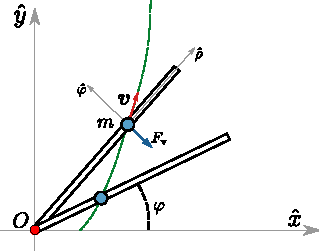
\includegraphics[width=0.4\textwidth]{images/fig_barra_giratoria.pdf}
	\end{center}
	\caption{Problema de la barra que gira con una masa $m$ enhebrada.}
	\label{fig_barra_giratoria}
\end{figure} 

Claramente la bola seguirá, con respecto a un sistema de coordenadas polar $(\rho,\vp)$ con origen en el punto $O$,
una trayectoria como la esquematizada por la curva verde. 
% Las coordenadas generalizadas son $\rho,\vp$

En este problema no hay potencial y el lagrangiano, que es $T$, será 
\[
	\Lag = \frac{1}{2} ( \dot{\rho}^2 + \rho^2 \omega^2 )
\]

El hamiltoniano es 
\be
	\Ham = \frac{1}{2} ( \dot{\rho}^2 - \rho^2 \omega^2 ).
	\label{ham_ejemplo_bola}
\ee
Luego, como el lagrangiano no depende explícitamente del tiempo entonces el hamiltoniano dado por la \eqref{ham_ejemplo_bola}
se conserva. No obstante, el hamiltoniano no es la energía puesto que la energía cinética $ T $ tiene la forma  $ T = T_2 + T_0 $,
que proviene del hecho de que la fuerza de vínculo (que tendrá dirección angular en este caso) dependerá del tiempo.
La energía no se conserva, claramente hay trabajo de la fuerza de vínculo, que es una fuerza no conservativa. 

La conservación del hamiltoniano dependerá de las coordenadas generalizadas elegidas. Podría pensarse que el $\Ham$ es la energía
vista en un sistema no inercial [?].
La energía siempre es la medida en un sistema inercial. Además, cuando se conserve lo será desde cualquier sistema de coordenadas
inercial elegido.
 
\end{ejemplo}


% =================================================================================================
\section{Energía cinética y el hamiltoniano}
% =================================================================================================

Dado que la energía cinética tiene la forma general
\[
	T = \underbrace{\frac{1}{2} \sum_i^N m_i \left( \dpar{\vb{r}_i}{t} \right)^2}_{T_0}  +
	\underbrace{\sum_j^{3n-k} b_j(q_1,...,q_{3N-k},t)\dot{q}_j  }_{T_1} +
	\underbrace{\frac{1}{2} \sum_j^{3n-k}\sum_s^{3n-k}  a_{js}(q_1,...,q_{3N-k},t)\dot{q}_s\dot{q}_j }_{T_2}
\]
entonces se sigue que 
\be
	E = T_0 + T_1 + T_2 + V
\label{mc_E}
\ee
y como 
\[
	p_i = \dpar{\Lag}{\dot{q}_i} = T_1 + 2T_2 
\]
es 
\[
	\Ham = \sum_i^N p_i\dot{q}_i - (T_0 + T_1 + T_2 - V) = 2T_2 + T_1 - T_0 - T_1 - T_2 + V = T_2 - T_0 + V
\]
pero como E es \eqref{mc_E} se tendrá 
\[
	E = H \iff 2T_0 + T1 = 0
\]
y un solución de este sistema es, por supuesto, $T_0 = T_1 = 0$

% =================================================================================================
\section{Principio de acción mínima}
% =================================================================================================

El estado de un sistema mecánico de $ N $ grados de libertad en un dado instante de tiempo $ t $ puede asociarse a 
un vector de componentes $ \{ q_i \} $ viviendo en un espacio $N$-dimensional de coordenadas generalizadas. 
La evolución entre dos puntos en ese espacio, de $ \{ q_i(t_a) \} $  a $ \{ q_i(t_b) \} $ por ejemplo, se realiza por
un trayecto continuo entre esos dos puntos, que es la trayectoria del sistema.

\begin{figure}[bth]
	\begin{center}
	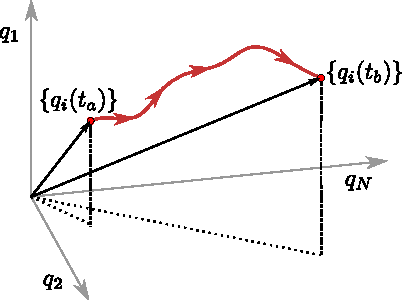
\includegraphics[width=0.5\textwidth]{images/fig_hamilton.pdf}	 
	\end{center}
	\caption{Trayectoria de un sistema mecánico $\{ q_i \}$ entre dos puntos del espacio $N$-dimensional de
	coordenadas generalizadas.}
	\label{principio_hamilton}
\end{figure}

En principio cualquier trayecto entre dos puntos es posible porque eso depende de la física a la cual está sometido
el sistema, no obstante existe un principio que permite saber cuál es la trayectoria que seguirá.

Considerando el lagrangiano $ \Lag = T - V $ y la siguiente integral (la acción $S$) entre los puntos $ \{ q_i(t_a) \} $
y $ \{ q_i(t_b) \} $,
\[
	S = \int_{t_a}^{t_b} \Lag( q_1(t, q_2(t), ..., \dot{q}_1(t),\dot{q}_2(t), ...,t )) \: dt
\]
se tiene que la trayectoria real entre estos dos puntos es tal que la integral $S$ toma su valor mínimo.

Dicho de otra manera, esto significa que $ S $ como funcional dependiendo de $ \{ q_i \}, \{ \dot{q}_i \} $
deberá tener un valor mínimo (o ser estacionaria) al especializarse en la trayectoria real.
Esto es análogo a lo que sucede en cálculo; en el mínimo de una función (de una o varias variables) la derivada 
se anula. El concepto equivalente en funcionales como $ S $ es el de variación nula.

La idea es construir una {\it variación} arbitraria respecto de la trayectoria real $ \{ q_i \} $ y forzar a que esa 
variación se anule para obtener un condición sobre las $ \{ q_i \} $ (para funciones esa condición era que el gradiente
se anule).

Si me sitúo en la trayectoria verdadera, es decir el conjunto $ \{ q_i(t) \}$, una variación arbitraria de la misma
tendrá la forma
\be
	q_i(t) \rightarrow q_i(t) + \delta q_i(t) \qquad i=1,2, ...
	\label{variacion}
\ee
donde cada coordenada $ q $ variará de acuerdo con su correspondiente desplazamiento $\delta q $.
La variación se hace en un intervalo de tiempo arbitrario $ [t_a,t_b] $ y con extremos fijos, 
\be
	\delta q(t_a) = 0 \qquad \qquad \delta q(t_b) = 0,
	\label{extremos_fijos}
\ee
lo que significa que los puntos de partida y llegada en el espacio de fases son los mismos.
\notamargen{Habría que justificar cuál es el significado de esto y porqué es así.}

Asimismo se pedirá que todas las trayectorias empleen el mismo tiempo de manera que la variación se hará en algún
tiempo fijo intermedio $ t_a < t < t_b $. O sea que $\delta t = 0$.

\notamargen{Cuán sketchi es todo esto!! Mucho para aclarar. Tal vez se justifique un minicurso de variacional como 
apéndice.}

Una representación unidimensional (una única $q$) puede verse en la Figura \ref{principio_accion_minima}.
La trayectoria real sería la curva $ q(t) $ en color rojo, mientras que la curva verde sería una trayectoria variada
a través de $ \delta q $. Los extremos fijos \eqref{extremos_fijos} implican que la variación es nula allí, y entonces
las curvas comienzan y terminan en el mismo punto.

\begin{figure}
	\begin{center}
	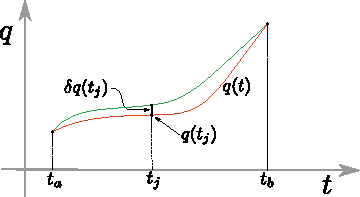
\includegraphics[width=0.7\textwidth]{images/fig_accion.pdf}	 
	\end{center}
	\caption{El principio de acción mínima}
	\label{principio_accion_minima}
\end{figure}

El hecho de considerar una variación a tiempo fijo $t_j$ implica que nos situaremos arbitrariamente en ese instante
y variaremos las trayectorias $ \{ q_i \} $ congeladas en ese instante arbitrario. Por supuesto, el resultado debería
valer para cualquier instante intermedio considerado.

La idea es determinar las condiciones que se necesitan para 
\[
	\frac{\delta S}{\delta q_i} = 0.
\]

Para ello comenzamos tomando una variación de $S$ que pasa dentro de la integral como 
\[
	\delta S = \int \left[ \Lag(q_i + \delta q_i, \dot{q}_i + \delta \dot{q}_i , t )
	- \Lag(q_i , \dot{q}_i , t ) \right] dt
\]
y donde vemos explícitamente que es a tiempo fijo.

La variación de la integral puede escribirse 
\[
	\delta S =  \int_{t_a}^{t_b} \sum_i^N \left( \dpar{\Lag}{\dot{q}_i} \delta \dot{q}_i +
	\dpar{\Lag}{q_i} \delta q_i  \right) dt,
\]
y como será útil tener todo en función de las variaciones $\delta q_i$, es conveniente expresar las variaciones $ 
\delta \dot{q}_i $ en términos de una derivada total a través de  
\[
	\frac{d}{dt}\left( \dpar{\Lag}{\dot{q}_i} \delta q_i \right) =
	\frac{d}{dt}\left( \dpar{\Lag}{\dot{q}_i} \right) \delta q_i + \dpar{\Lag}{\dot{q}_i}\delta \dot{q}_i,
\]
resultando en 
\[
	\delta S =  \int_{t_a}^{t_b} \sum_i^N \left[ \frac{d}{dt}\left( \dpar{\Lag}{\dot{q}_i} \delta q_i \right) -
	\frac{d}{dt}\left( \dpar{\Lag}{\dot{q}_i} \right) \delta q_i + \dpar{\Lag}{q_i} \delta q_i  \right] dt,
\]
que se puede separar en dos términos
\[
	\delta S =  \int_{t_a}^{t_b} \sum_i^N \left[ \frac{d}{dt}\left( \dpar{\Lag}{\dot{q}_i} \delta q_i \right) 
	\right] dt + \int_{t_a}^{t_b} \sum_i^N \left[ \dpar{\Lag}{q_i} - \frac{d}{dt}\left( \dpar{\Lag}{\dot{q}_i} 
	\right) \right]  \delta q_i \; dt,
\]

Pero el primer término es una derivada total y por el teorema fundamental del cálculo,
\be
	\int_{t_a}^{t_b} \sum_i^N \left[ \frac{d}{dt}\left( \dpar{\Lag}{\dot{q}_i} \delta q_i \right) \right] dt =
	\sum_i^N \left. \dpar{\Lag}{\dot{q}_i} \delta q_i \: \right|_{t_a}^{t_b}
\label{mc_borde_term}
\ee
y es nulo porque $\delta q_i=0$ en los extremos para toda coordenada $i$ (las variaciones son nulas en los extremos). 
Decimos que este es un término de superficie. Entonces la condición 
\[
	\delta S =  \sum_i^N  \int_{t_a}^{t_b}
	\left[ \dpar{\Lag}{q_i} - \frac{d}{dt}\left( \dpar{\Lag}{\dot{q}_i} \right)  \right]  \delta q_i  dt = 0
\]
se verificará por el cumplimiento de las ecuaciones de Euler-Lagrange\footnote{Como las variaciones $\delta q_i$ son 
arbitrarias e independientes la anulación de la ecuación $ \delta S $ requiere la anulación de cada uno de los 
$i=1,2,...N $ corchetes en los integrandos.}
\[
	\sum_i^N  \left[ \frac{d}{dt}\left( \dpar{\Lag}{\dot{q}_i} \right) - \dpar{\Lag}{q_i} \right] = 0.
\]

Se puede ver que 
\[
	\delta S = 0 \quad \iff \quad \sum_i^N  \left[ \frac{d}{dt}\left( \dpar{\Lag}{\dot{q}_i} \right) -
	\dpar{\Lag}{q_i} \right] = 0.
\]


Luego, si se hace $\Lag' = \Lag + df/dt$ (ambos lagrangianos difieren en una derivada total con 
respecto al tiempo) la trayectoria que minimiza $\Lag'$ es la que misma que minimiza
$\Lag$ por la condición dada por \eqref{mc_borde_term}. 

La moraleja es que si los lagrangianos difieren en una derivada total del tiempo obtenemos la misma
física.

\begin{ejemplo}{\bf Problema círculos}

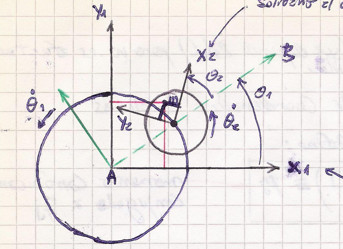
\includegraphics[scale=0.3]{images/fig_mc_dos_circulos_rotantes.jpg} 
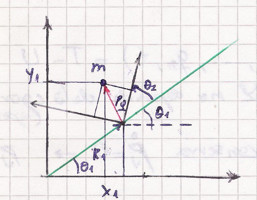
\includegraphics[scale=0.3]{images/fig_mc_dos_circulos_subsistema.jpg} 
 
El disco pequeño está solidario al disco [?]. La línea AB está pintada sobre los discos para poder medir los ángulos.
El eje $x_1$ está solidario al piso (inercial).

La segunda figura ilustra el movimiento de la masa en el sistema fijo.,
\[
	x_1 = R_1 \cos \theta_1 + \rho \cos ( \theta_1 + \theta_2 + \vp )
\]
\[
	y_1 = R_1 \sin \theta_1 + \rho \sin ( \theta_1 + \theta_2 + \vp )
\]
Luego, hay que calcular 
\[
	\frac 1 2 m |\vb{v}|^2
\]
con 
\[
	\dot{x}_1 = -R_1 \sin \theta_1 \dot{\theta}_1 + \dot{\rho} \cos ( \theta_1 + \theta_2 + \vp ) -
	\rho ( \dot{\theta}_1 + \dot{\theta}_2 + \dot{\vp} ) \sin( \theta_1 + \theta_2 + \vp )
\]
\[
	\dot{y}_1 = R_1 \cos \theta_1 \dot{\theta}_1 + \dot{\rho} \sin ( \theta_1 + \theta_2 + \vp ) +
	\rho ( \dot{\theta}_1 + \dot{\theta}_2 + \dot{\vp} ) \cos( \theta_1 + \theta_2 + \vp )	
\]

Habría que elevar esto al cuadrado, lo cual a mano es un trabajo un poco cumbersome.
\[
	T = \frac 1 2 m ( R_1^2 \dot{\theta}_1^2 + \rho^2( \dot{\theta}_1 + \dot{\theta}_2  + \dot{\vp} ) + \dot{\rho}^2 + 
	2R_1\dot{\theta}_1\left[ \dot{\rho}\sin(\theta_2+\vp) + \rho( \dot{\theta}_1 + \dot{\theta}_2 + \dot{\vp} )\cos(\theta_2+\vp) \right])
\]
y como no hay potencial, entonces $\Lag = T $. Trabajando con las ecuaciones de Lagrange se llega a
\[
	\ddot{\rho} - \rho ( \omega_1 + \omega_2 + \dot{\vp} )^2 - R_1 \omega_1^2 \cos (\omega_2 t + \vp ) = 0
\]
\[
	\ddot{\vp} + \frac{\dot{\rho}}{\rho}\left[ 2(\omega_1 + \omega_2 )\right] + 
	\frac{R_1\omega_1( \omega_1 + \omega_2 )}{\rho} \sin (\omega_2 t + \vp ) = 0
\]

Este sistema tiene dos grados de libertad $(\rho,\vp)$ y el lagrangiano es $\Lag(\vp,\rho,\dot{\vp},\dot{\rho},t)$. En realidad
$\dot{\theta}_j = \dot{\theta}_j(\rho\vp)$ para $j=1,2$ y entonces $\theta_j$ no son coordenadas generalizadas.

Este problema se puede simplificar si se asume que $ \dot{\theta}_1, \dot{\theta}_2 $ son constantes [Esto viene antes o viene después].
\end{ejemplo}


\begin{ejemplo}{\bf Problema 17}
 
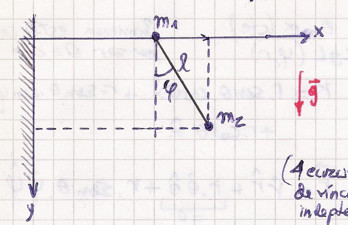
\includegraphics[scale=0.3]{images/fig_mc_pendulo_deslizante.jpg} 

Un problema de dos masas con, en principio, seis grados de libertad. Dado que el movimiento se asume que ocurre en un plano, el $z$
por ejemplo, eso implica dos vínculos $z_1 = z_2 = 0$ a los cuales debemos sumarle la fijación de $m_1$ en la altura $y_1 = 0$ y el vínculo 
de la barra
\[
	y_2^2 + (x_2 -x_1)^2 = \ell^2
\]
luego es un problema de dos grados de libertad, que pueden ser elegidos como $(x,\vp)$. Esto último puesto que 
\[
	x_2 = x + \ell \sin\vp \qquad y_2 = \ell \cos \vp.
\]
Considerando $x_1 equiv x$ para simplificar la notación se tiene 
\[
	\dot{x}_2 = \dot{x} + \ell \dot{\vp}\cos\vp \qquad \qquad \dot{y}_2 = -\ell \dot{\vp} \sin\vp
\]

Todo esto permite escribir 
\[
	T = \frac 1 2 ( m_1 + m_2 ) \dot{x}^2 + \frac 1 2 m_2 ( 2\dot{x}\dot{\vp} \ell\cos\v + \ell^2\dot{\vp}^2 )
\]
\[
	V = - m_2 g \ell \cos\vp
\]
La condición de que $\Lag \neq \Lag(\vp)$ implica la cantidad conservada
\[
	\dpar{\Lag}{\dot{x}} = \dot{x}(m_1+m_2) + m_2 \dot{\vp} \ell \cos\vp \equiv p_x,
\]
que es el momento lineal en $x$. Para la coordenada $\vp$ resulta la ecuación
\[
	\ddot{x}\cos\vp + \ell\ddot{\vp} + g\sin\vp = 0,
\]
mientras que para $x$ se tiene 
\[
	\ddot{x}(m_1+m_2) + m_2 \ell (\cos \vp \ddot{\vp}-\sin\vp \dot{\vp}^2)	= 0.
\]

Se pueden combinar para tener una ecuación para $ \vp $ solamente. Luego esa dinámica la puedo obtener? [ver carpeta].
\end{ejemplo}


\begin{ejemplo}{\bf Problema 7}
 
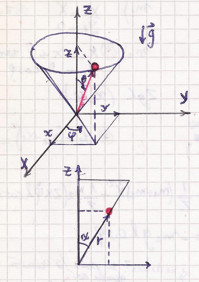
\includegraphics[scale=0.35]{images/fig_mc_problema_cono.jpg}

En este problema convienen esféricas $\theta$ constante. Tendremos dos grados de libertad $(\varphi,r)$.
Usando las expresiones de las coordenadas esféricas (ver XXXX chap 1) se tiene 
\[
	| \dot{\vb{x}} |^2 = | \dot{r}\hat{r} + r\sin\theta \dot{\vp} \hat{\vp} |^2
\]
\[
	v^2 = \dot{r}^2 + r^2 \dot{ \vp }^2 \sin^2 \alpha
\]
Con esto escribimos $T$ usando que $V = mgr\cos\alpha$,
\[
	\Lag = \frac 1 2 m (\dot{r}^2 + r^2 \dot{ \vp }^2 \sin^2 \alpha) - mgr \cos\alpha 
\]

El grado de libertad $\vp$ tendrá asociado un momento conjugado que se conserva, pues $\partial\Lag/\partial \vp = 0$,
luego
\[
	\dpar{\Lag}{\dot{\vp}} = mr^2 \dot{\vp} \sin^2 \alpha = cte. \equiv L
\]
mientras la ecuación de E-L para $r$ arrojará
\[
	m\ddot{r} - m r \dot{\vp}^2 \sin^2\alpha + mg\cos\alpha = 0
\]
y utilizando la conservación 
\[
	\ddot{r} - \frac{L^2}{mr^3\sin^2\alpha} + mg\cos\alpha = 0.
\]

Si ahora calculamos la energía $E=T+V$ se obtiene 
\[
	E = \frac 1 2 m \dot{r}^2 + \frac{L^2 \vp}{ m r^2 \sin^2 \alpha } + mgr\cos\alpha
\]
donde los dos últimos términos constituyen un potencial efectivo.
 
\end{ejemplo}

\begin{ejemplo}{\bf Cicloides y esas cosas}
Tautocrona, Huygens (1773)

\subsubsection*{Curva cicloide}

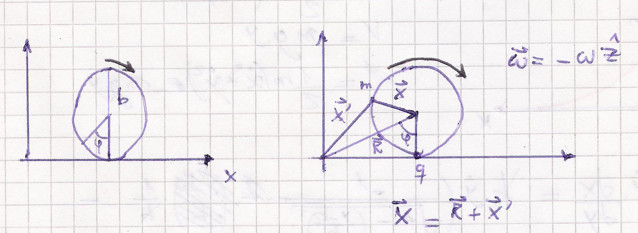
\includegraphics[scale=0.3]{images/fig_mc_cicloides.jpg}

Con las consideraciones de las figuras, tenemos en rápida sucesión
\[
	\vb{R} = (vt,b)
\]
\[
	\vb{X}' = ( -b \sin \vp, -b \cos \vp ) ; \quad \vp = \omega t
\]
\[
	\vb{X} = ( vt -b \sin \vp, b -b \cos \vp )
\]
y por condición de rodadura
\[
	\vb{v}_q = 0 = \vb{v}_{cm} + \vb{\omega} \times \vb{x}_{cm} = v\hat{x} + (-\omega)b\hat{k} \times (-\hat{y})
\]
\[
	0 = (v-\omega b)\hat{x},
\]
o bien $v=\omega b$ e integrando
\[
	vt = \omega t b = \vp b.
\]

Con esto llego a mi ecuación paramétrica para el cicloide
\[
	\begin{cases}  x = b \: (\vp - \sin \vp )\\
		       y = b \: (1 - \cos \vp )
	\end{cases}
\]
Este cicloide tiene gráfico 

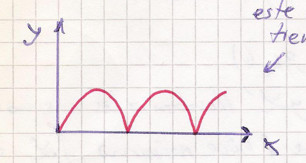
\includegraphics[scale=0.2]{images/fig_mc_cicloide_tiny.jpg}
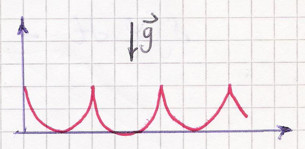
\includegraphics[scale=0.2]{images/fig_mc_cicloide_tiny_inverted.jpg}

Pero neceisto uno que mire hacia abajo, lo cual se logra con un cambio $y' = -y + bz $ de modo que 
\[
	\begin{cases}  x = b \: (\vp - \sin \vp )\\
		       y = b \: (1 + \cos \vp )
	\end{cases}
\]

Ahora se hace un cambio de variables nuevo 
\[
	\frac y b = 1 + \cos\vp \qquad \qquad \frac{y-b}{b} = \cos \vp
\]
y entonces
\[
	x(y) = b \left( \acos\left( \frac{y-b}{b} \right) - \sqrt{1 - ( (y-b)/b )^2} \right)
\]

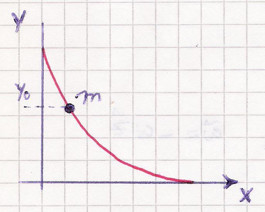
\includegraphics[scale=0.2]{images/fig_mc_cicloide_tobogan.jpg}

Usando todo esto
\[
	T = \frac 1 2 m ( \dot{x}^2 + \dot{y}^2 ) \qquad \qquad V = m g y
\]
\[
	\Lag = \frac 1 2 m ( \dot{x}^2 + \dot{y}^2) - mgy
\]
Derivando $x$ y haciendo el álgebra,
\[
	\dot{x} = -\dot{y} \sqrt{ \frac{ 2b - y }{y} }.
\]

Utilizando toda esta información, el lagrangiano es
\[
	\Lag = \frac{mb\dot{y}}{y} - mgy
\]
y las ecuaciones de E-L
\[
	mb\left( 2\frac{\ddot{y}}{y} - \frac{\dot{y}^2}{y^2} \right) + mg = 0.
\]

Podemos ver, con alguna experiencia, que 
\[
	\dtot{}{t}\left( \frac{ \dot{y}^2 }{y} \right) = \dot{y} \left( 2 \frac{ \ddot{y} }{y} - \frac{\dot{y}^2}{y^2} \right)
\]

Luego,
\[
	m b \frac{1}{\dot{y}} \dtot{}{t}\left( \frac{ \dot{y}^2 }{y} \right) + m g = 0
\]
\[
	\dtot{}{t}\left( \frac{ \dot{y}^2 }{y} \right) = - \frac{ g }{ b } \dtot{y}{t},
\]
y ahora se puede integrar
\[
	\int_0^t \dtot{}{t}\left( \frac{ \dot{y}^2 }{y} \right) dt = 
	- \frac{ g }{ b } \int_0^t \dtot{y}{t} dt,
\]
\[
	\left. \frac{ \dot{y}^2 }{y} \right|_0^t = - \left. \frac{ g }{ b } y \right|_0^t
\]

Usando condiciones iniciales
\[
	\begin{cases}
	 \dot{y}(t=0) = 0 \\
	 y(t=0) = y_0
	\end{cases}
\]
\[
	\frac{ \dot{y}^2 }{ y } = -\frac{ g }{ b } y +  \frac{ g }{ b } y_0
\]
\[
	\dot{y} = \frac{g}{b} \sqrt{ (y_0 - g) y }
\]
de manera que 
\[
	\int_{y_0}^{y} \frac{ dy }{ \sqrt{ y_0y - y^2 } } = \sqrt{ \frac g b } \int_0^t dt = \sqrt{ \frac g b } t
\]
\[
	\asen\left( \frac{ y - y_0/2 }{y_0/2} \right)|_{y_0}^y = \asen\left( \frac{y - y_0/2}{y_0/2} \right)  - \frac \pi 2
\]
\[
	\frac{y - y_0/2}{y_0/2} = \sin ( \sqrt{ \frac g b } t + \pi/2 ) = \cos ( \sqrt{ \frac g b } t )
\]
Finalmente,
\[
	y(t) = \frac {y_0} 2 ( 1 + \cos ( \sqrt{ \frac g b } t ) ).
\]

Si quiero calcular el tiempo de caída será:
\[
	0 = \frac{y_0}{2}\left( 1 + \cos ( \sqrt{ \frac g b } \tau ) \right),
\]
de lo cual se deduce 
\[
	\tau = \sqrt{ \frac b g } \pi.
\]

La cicloide es la curva de caída por la cual se tarda el tiempo mínimo. La masa $m$ tarda lo mínimo en caer por esta curva.
Si las dos ruedas están pegadas girando ambas, recorrerán en un giro una distancia verde:

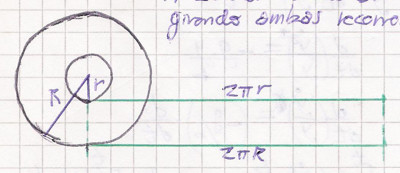
\includegraphics[scale=0.2]{images/fig_mc_ruedas_pegadas.jpg}

Esto no sucede: alguna de ambas deslizará.
\end{ejemplo}




% =================================================================================================
\section{Aplicaciones del principio de acción mínima}
% =================================================================================================

\notamargen{Me falta algo de esta clase inicial, pero esperamos que no sea fundamental!}
El principio variacional de Hamilton tiene más uso como herramiento formal de lo que tiene en el campo de la aplicación.

\[
	S = \int (T-V_0) dt
\]
donde el lagrangiano es con $V=V_0$ constante (un lagrangiano sujeto a potencial constante).
La integral de acción da una medida de la longitud de la órbita (el espacio recorrido).
Para una partícula sujeta a $V=0$
\[
	S = \frac{1}{2}\int m v_0^2 dt = \frac{1}{2}mv_0^2(t-t_0)
\]
de manera que $v_0(t-t_0)$ representa la distancia $d$ recorrida, y es 
\[
	S = \frac{1}{2}mv_0 d
\]

Comentario sobre el cálculo de las variaciones
\notamargen{Esta idea debe estar en el suplemento matemático que le dedicaremos a variacional}
\[
	I = \int f\left(x, \dtot{x}{t}, t\right) dt 
\]
entonces $I$ es extremo si
\[
	\frac{d}{dt} \left( \dpar{f}{[dx/dt]}\right) - \dpar{f}{x} = 0
\]
También podemos encontrar esta notación, dependiendo del tipo de problema,
\[
	I = \int f\left(y, \dtot{y}{x}, x\right) dx 
\]

\subsection{Billares [otro título?]}

Consideramos una partícula libre en una región del espacio (una partícula rebotando en cierta región). Podemos pensar en un
potencial 
\[
	V(\vb{x}) = \begin{cases}
	0\phantom{\infty} \quad \vb{x} \in D \\
	\infty\phantom{0} \quad \vb{x} \notin D
	\end{cases}
\]
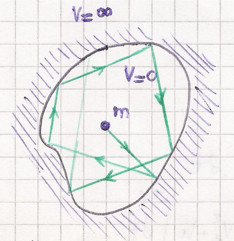
\includegraphics[scale=0.3]{images/fig_mc_billar_1.jpg}

Es un pozo de potencial con una partícula libre en su interior; se los suele llamar {\it billares}. En este caso
\[
	I = \int_{q_i}^{qa_f} \: \Lag( q_1(t), q_2(t), ..., q_k(t),\dot{q}_1(t), ..., \dot{q}_k(t), t ) dt.
\]
La integral da la longitud de la órbita (espacio recorrido)
\[
	\frac 1 2 m v_0^2 \int_{t_i}^{t_f} dt = \frac 1 2 m v_0^2 (t_f - t_i)
\]

En un billar circular 

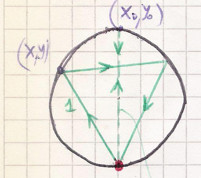
\includegraphics[scale=0.3]{images/fig_mc_billar_2.jpg}
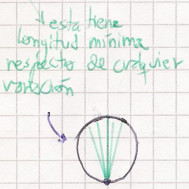
\includegraphics[scale=0.3]{images/fig_mc_billar_2b.jpg}

Si parto del punto rojo y quiero minimizar (extremar) la trayectoria que me da el ir hacia $(x,y)$ y volver al punto rojo, obtendré
una órbita periódica en $(x_0,y_0)$. Esa órbita periódica es extrema entre ir y volver al punto rojo.

En un billar eliptico

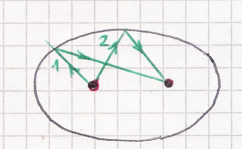
\includegraphics[scale=0.3]{images/fig_mc_billar_3.jpg} 

hay muchas trayectorias posibles entre los focos.
El lagrangiano integrado me da todos las extremas $(1,2,...)$, que por otro lado son las reales, y con las condiciones iniciales determinaré qué 
trayectoria extrema estaré considerando.

Hay muchas trayectorias $(1,2,...)$ que son posibles 

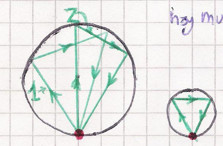
\includegraphics[scale=0.3]{images/fig_mc_billar_4.jpg} 

\[
	I = \int \Lag
\]
da la longitud total de todo el camino.
\notamargen{¿Esta sección aporta algo?}


\subsection{Minimización del camino entre dos puntos}

\notamargen{Esto lo clavo por acá, después reacomodarlo}

\begin{figure}[htb]
	\begin{center}
	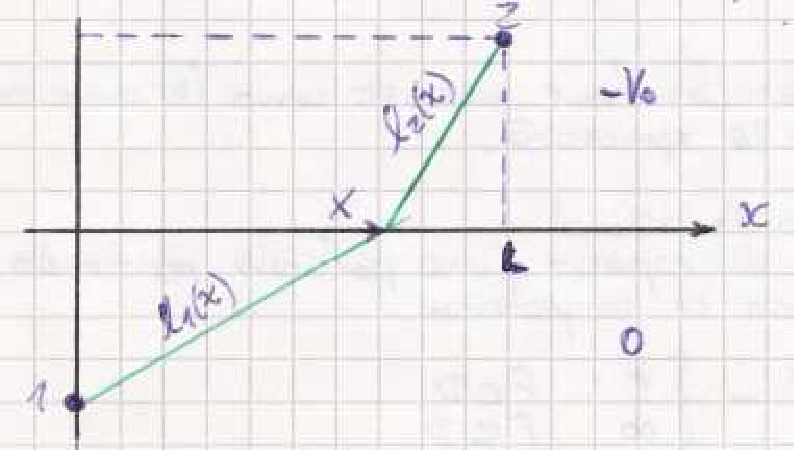
\includegraphics[width=0.4\textwidth]{images/fig_mc_snell1.pdf}	 
	\end{center}
	\caption{}
	\label{fig_mc_snell1}
\end{figure}

El $ \tau $ es fijo.
Este problema no es como el del billar porque la velocidad no es constante [?].
\[
	I = \int_1^2 \Lag \: dt 
\]
pero se puede descomponer en $ I = I_1 + I_2 $; es decir un lagrangiano para cada medio, luego
\[
	I = \frac{1}{2} m v_1^2 \int_0^{t_i} dt + (\frac{1}{2} m v_2^2 + V_0) \int_{t_i}^{t_f} dt ,
\]
que al integrar da
\[
	I = \frac{1}{2} m v_1^2 t_i + \frac{1}{2} m v_2^2( t_f - t_i ) + V_0( t_f - t_i ).
\]

Las condiciones geométricas del problema (ver Figura) implican que 
\[
	v_1 t_i = \ell_1(x) \qquad \qquad v_2 ( t_f - t_i ) = \ell_2(x)
\]
siendo $ \ell_i $ longitudes que dependen de $ x $. Esto permite expresar los tiempos $t$ en términos
de la distancia $ x $ sobre la frontera. Entonces se obtiene la acción $I$ en términos de posiciones
y velocidades, i.e.
\[
	I = I(v_1,v_2 ,x) = \frac{1}{2} m v_1 \ell_1(x) + \frac{1}{2} m v_2 \ell_2(x) + \frac{V_0}{V_2} \ell_2(x).
\]

Luego, como todo sucede a $\tau$ fijo ($t_f=\tau$) se debe tener el siguiente vínculo
\[
	\tau = \frac{\ell_1(x)}{v_1} + \frac{\ell_2(x)}{v_2}.
\]
Entonces, diferenciando implícitamente el vínculo y la integral $I$ obtenemos, respectivamente,
\[
	d\tau = 0 = \left( \frac{1}{v_1} \dtot{\ell_1}{x} + \frac{1}{v_2} \dtot{\ell_2}{x} \right) dx
	-\frac{\ell_1}{v_1^2} dv_1 - \frac{\ell_2}{v_2^2}dv_2
\]
\[
	dI = \left(  \frac{v_1}{2} \dtot{\ell_1}{x} +  \frac{v_2}{2} \dtot{\ell_2}{x} + 
	 \frac{V_0}{v_2} \dtot{\ell_2}{x} \right) dx + 
	\frac{\ell_1}{2} dv_1 + \left( \frac{\ell_2}{2} - \frac{V_0 \ell_2}{v_2^2} \right)dv_2 = 0
\]
En esta última ecuación, si fuesen independientes los diferenciales $dx,dv_1,dv_2$ entonces sería nulo cada
paréntesis. Como no es el caso empleamos multiplicadores de Lagrange,
\[
	d\tau = \lambda \left( \frac{1}{v_1} \dtot{\ell_1}{x} + \frac{1}{v_2} \dtot{\ell_2}{x} \right) dx
	- \lambda \frac{\ell_1}{v_1^2} dv_1 - \lambda \frac{\ell_2}{v_2^2}dv_2
\]
y combinando
\begin{multline*}
 	\left(  \frac{v_1}{2} \dtot{\ell_1}{x} +  \frac{v_2}{2} \dtot{\ell_2}{x} + 
	 \frac{V_0}{v_2} \dtot{\ell_2}{x} - \lambda \left[ \frac{1}{v_1} \dtot{\ell_1}{x} + \frac{1}{v_2} 
	\dtot{\ell_2}{x}  \right] \right) dx + \\
	\left( \frac{\ell_1}{2} + \lambda \frac{\ell_1}{v_1^2} \right) dv_1 + 
	\left( \frac{\ell_2}{2} - \frac{V_0 \ell_2}{v_2^2} + \lambda \frac{\ell_2}{v_2^2} \right)dv_2.
\end{multline*}

Ahora se puede igualar a cero cada paréntesis porque consideramos independientes $v_1$ y $v_2$.
Entonces, se tienen
\[
	\lambda = -\frac{1}{2}v_1^2 \qquad \qquad \lambda = -\frac{1}{2}v_2^2 + V_0
\]
de manera que ha resultado la conservación de la energía
\[
	\frac{1}{2}v_1^2 = \frac{1}{2}v_2^2 - V_0
\]

Reemplazando en la anterior expresión, se llega a
\[
	v_1 \dtot{\ell_1}{x} + v_2 \dtot{\ell_2}{x} = 0.
\]

\[
	\ell_1 = \sqrt{ Y_0^2 + x^2 } \qquad \ell_2 = \sqrt{ Y_f^2 + (L-x)^2 }
\]
\[
	\dtot{\ell_1}{x} = \sin(\alpha_1) \qquad \dtot{\ell_2}{x} = -\sin(\alpha_2)
\]
de modo que 
\[
	v_1 \sin( \alpha_1 ) = v_2 \sin( \alpha_2 ),
\]
que es la conclusión de la ley de Snell. Entonces podemos establecer un parangón entre mecánica clásica
y óptica geométrica.

\begin{figure}[htb]
	\begin{center}
	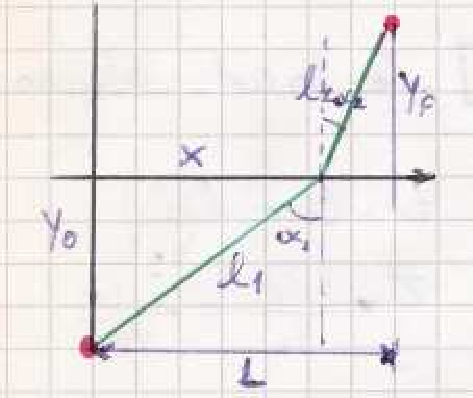
\includegraphics[width=0.4\textwidth]{images/fig_mc_snell2.pdf}	 
	\end{center}
	\caption{}
	\label{fig_mc_snell2}
\end{figure}

\subsection{Acción mínima ejemplos}

En general, dada una integral
\[
	I = \int_{t_1}^{t_2} \: f\left(y,\dtot{y}{t},t\right) \: dt,
\]
si se tiene que 
\[
	\dtot{}{t}\left( \dpar{f}{dy/dt} \right) - \dpar{f}{y} = 0,
\]
entonces se da que $I$ es un extremo. Por ello esta idea es generalizable a casos no mecánicos, como veremos a 
continuación.

\begin{ejemplo}{\bf Espejimo -problema 5-}
 
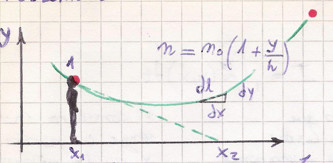
\includegraphics[scale=0.3]{images/fig_mc_espejismo.jpg}

En estos problemas debemos saber primeramente de qué punto a qué punto vamos.
\[
	I = \int_{x_1}^{x_2} n(y) d\ell = \int_1^2 n_0 \left( 1 + \frac y h \right) \sqrt{ dx^2 + dy^2} =
	\int_1^2 n_0 \left( 1 + \frac y h \right) \sqrt{ 1 + \left( \frac{dy}{dx} \right)^2 } \: dx
\]
Si defino $ y' = dy/dx$ y $f = n_0 (1 + y/h) \sqrt{ 1 + {y'}^2}$ se tiene 
\[
	\dtot{}{x}\left( \dpar{f}{y'}\right) = \dtot{}{x} \left( n_0 \left( 1 + \frac y h \right) 
	\frac{y'}{\sqrt{ 1 + {y'}^2}} \right)
\]
y haciendo la derivada explícitamente
\[
	\dtot{}{x}\left( \dpar{f}{y'}\right) = n_0 \left( 
	\frac{ {y'}^2}{h\sqrt{1 + {y'}^2} } + \left( 1 + \frac y h \right) 
	\left[ y''\frac{1}{\sqrt{1 + {y'}^2}} + \frac{y'}{2 (\sqrt{1 + {y'}^2})^3 } 2 y' y'' \right]
	\right)
\]
\[
	\dpar{f}{y} = \frac {n_0}{h}  \sqrt{ 1 + { y'}^2 } 
\]
Luego, juntando todo
\[
	y'' = \frac{1 + y'^2}{h+y}.
\]

Si tomamos 
\[
	y + h = \frac{\alpha h}{n_0} \cosh \left( \frac{\alpha n_0}{\alpha h}+ \beta \right)
\]
\[
	y'' = \frac{n_0}{\alpha h} \cosh ()
\]
\notamargen{Acá, claramente, faltan cosas.}
\end{ejemplo}

\begin{ejemplo}{\bf Problema 8}

Por la periodicidad se propone una serie de Fourier
\[
	y = \frac{a_0 }{2} + \sum_{n=1} a_n \cos (n\omega t) + b_n \sin (n\omega t)
\]
donde $\omega$ corresponde a la frecuencia del movimiento de subida y bajada.
\[
	y(0) = 0 \qquad \qquad \Lag = T - V
\]
\[
	y(t_{\text{caida}}) = 0 \qquad \qquad \Lag = \frac m 2 \dot{y}^2 - m g y
\]
Entonces queremos lograr $\delta I = 0$ para 
\[
	I = \int_0^{t_c}  \: \Lag \: dt
\]
para hallar la mejor serie de Fourier que verifique
\[
	\dot{y} = \sum_{n} - a_n \sin (n\omega t) n \omega + b_n \cos (n\omega t) n\omega
\]
y esto habría que elevarlo al cuadrado.

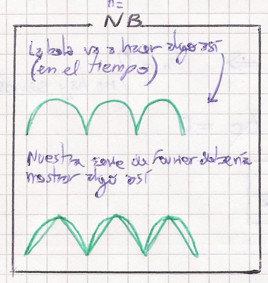
\includegraphics[scale=0.3]{images/fig_mc_fourier_1.jpg}
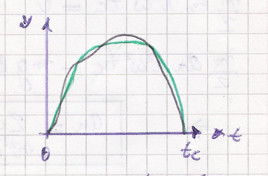
\includegraphics[scale=0.3]{images/fig_mc_fourier_2.jpg}

Quisiera ver la diferencia entre las dos trayectorias que muestra la figura.
\[
	y(0) = \frac{ \omega }{2} + \sum a_n = y( t_c )
\]
Y calculo acá las variaciones
\[
	0 = \delta y(0) = \delta \frac{a_0}{2} + \sum_n \delta a_n
\]
\[
	\delta a_0 = - \sum_n 2 \delta a_n \qquad   \text{vinculo}
\]
\[
	I = m \int_0^{t_c} \left[ \sum_n a_n n \omega \sin( n\omega t) + b_n n\omega \cos (n\omega t) \right]^2 dt 
	- mg \int_0^{t_c} \left[ \frac {a_0} 2 \sum_n a_n \cos( n\omega t) + b_n \sin (n\omega t) \right] dt
\]
\notamargen{Anoté: porque $t_c$ es el tiempo de un período.}
\[
	\int_0^{t_c} \cos (n\omega t) dt = 0 \qquad \qquad \int_0^{t_c} \sin (n\omega t) dt = 0
\]
\[
	\int_0^{t_c} \cos^2 (n\omega t) dt = T/2 \qquad \qquad \int_0^{t_c} \sin^2 (n\omega t) dt = T/2
\]
\[
	I = \frac m 2 \left( \sum_n a_n^2 n^2 \omega^2 \frac {T_c}2 + \sum_n b_n^2 n^2 \omega^2 \frac {T_c}2 \right) - m g T_c \frac {a_0} 2
\]

La integral ya está dada en función de los coeficientes de la serie, de manera que lo que faltaría es hacer variar los coeficientes y ya.
\[
	\delta I = - \frac m 2 \sum_n a_n \delta a_n n^2 \omega^2 t_c + \frac m 2 \sum_n b_n \delta b_n n^2 \omega^2 t_c -
	m g \delta \frac {a_0} 2 t_c + \frac{mg }{2} \sum_n 2 \delta a_n t_c = 0
\]
y como los $\delta a_n, \delta b_n$ son independientes todos los términos serán cero por separado.
Entonces
\[
	\frac m 2 b_n \delta b_n n^2 \omega^2 t_c = 0 \qquad \qquad \Rightarrow \quad b_n= 0,
\]
es decir que no hay senos. Por otro lado,
\[
	a_n  = \frac {2g}{n^2\omega^2}
\]
y
\[
	y(t) = \sum_n \frac{1-\cos(n\omega t)}{n^2\omega^2/2g}
\]

Se ve que la mejor serie de Fourier tendrá algo que se aproxima a la parábola.

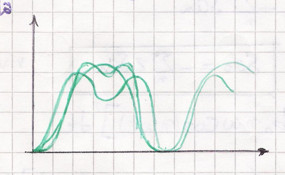
\includegraphics[scale=0.3]{images/fig_mc_fourier_3.jpg}

Podemos ver si se llega a la altura máxima $y_\text{maxima} \equiv y(t_c/2)$
\[
	y(t_c/2) = \frac{2g}{\omega^2}\sum_n \frac{2}{n^2} = \frac{4g}{\omega^2}\frac{\pi^2}{6} = \frac{gt_c^2}{6} = \frac{2v_0^2}{3g}
\]
o bien 
\be
	y(t_c/2) = \frac{2v_0^2}{3g}
	\label{sol_series_fourier}
\ee
donde 
\[
	E = mgy_\text{maxima}, E_0 = \frac{mv_0^2}{2}
\]
y la altura máxima real es $Y_\text{maxima} = v_0^2/(2g)$ que difiere de la que se obtiene con la serie de Fourier.
Entonces, la mejor solución de entre las series de Fourier es \eqref{sol_series_fourier} que difiere de la solución real.
Esta solución es derivable en los nodos, mientras que la solución real no lo es.
\notamargen{Este ejemplo hay que trabajarlo bastante!}
\end{ejemplo}

% =================================================================================================
\section{Multiplicadores de Lagrange}
% =================================================================================================

El principio variacional de Hamilton nos dice que la trayectoria real que sigue un sistema es la que 
extremiza la acción
\[
	S = \int_{t_i}^{t_f} \Lag \left( q_i[t], \dot{q}_i[t], t \right) dt.
\]
\notamargen{Habría que tomarse medio minuto para chequear: consistencia de la notación con respecto a los límites
en estas integrales de acción, definir extremización, ver si la implicancia es un sí y sólo sí o no, etc.}
Esa condición de extremo, conducía directamente a las ecuaciones de Euler-Lagrange, es decir
\be
	\delta S = 0 \quad \Leftrightarrow \quad \int \sum_{j=1}^{N} 
	\left[ \frac{d}{dt}\left( \dpar{\Lag}{\dot{q}_j} \right) - \dpar{\Lag}{q_j} \right]\delta q_j \: dt = 0
	\label{accion_nula_ecsel}
\ee
donde $\delta q_j$ eran desplazamientos independientes y esta condición significaba que el corchete debía
ser nulo para todo grado de libertad $j$.

Pero puede suceder (en el caso de vínculos no-holónomos, por ejemplo) que no se pueda despejar alguna $ q_j $ y 
entonces no todos los  $\delta q_j$ son independientes.

Si se tienen $s$ ecuaciones de vínculo no holónomos [¿cómo es un vínculo no-holónomo? o es que se deriva una
ecuación de vínculo usual??]
% y se las deriva con respecto al tiempo obtenemos
\[
	\sum_{\ell}^N a_\ell^k(q_i,t) \dot{q}_\ell + b^k(q_i,t) = 0 \qquad \qquad k=1,2,...,s
\]
donde $\ell$ suma en los grados de libertad.
% que son los vínculos ($k=1,...,s$); son $s$ ecuaciones de vínculo.
Multiplicando por $\delta t$ puede verse que no son independientes,
\[
	\sum_{\ell}^N a_\ell^k(q_i,t) \delta {q}_\ell + b^k(q_i,t) \delta t= 0 .
\]

Si ahora las $\delta q_\ell$ son variaciones a $t$ fijo, entonces se cumple 
\[
	\sum_{\ell}^N a_\ell^k(q_i,t) \delta {q}_\ell = 0,
\]
expresión que puede intregrarse con respecto al tiempo y sumar sobre todas las ecuaciones de vínculo,
\[
	\sum_{k}^s \int_{t_i}^{t_f} \lambda^k \sum_{\ell}^N a_\ell^k(q_i,t) \delta {q}_\ell \: dt = 0.
\]

El cero de esta última ecuación puede restarse del otro cero dado por la integral \eqref{accion_nula_ecsel},
suma de $N-s$ ecuaciones con $\delta q_\ell$ independientes [¿checar esto?] con para construirnos de esa manera la ecuación
% Podemos sacar la suma fuera,
% \[
% 	\sum_{k}^s \int_{t_i}^{t_f} \lambda^k \sum_{\ell}^N a_\ell^k(q_i,t) \delta {q}_\ell dt = 0
% \]
% Absorbo la otra sumatoria en el segundo término y paso de $\ell \to j$.
\[
	\int \sum_{j=1}^{N-s} \left\{ \frac{d}{dt}\left( \dpar{\Lag}{\dot{q}_j} \right) -\dpar{\Lag}{q_j}
	- \sum_{k}^s \lambda^k a_j^k(q_i,t) \right\} \delta {q}_j \: dt = 0
\]
y se tienen $N-s$ ecuaciones
\[
	\frac{d}{dt}\left( \dpar{\Lag}{\dot{q}_j} \right) -\dpar{\Lag}{q_j} =  \sum_{k}^s \lambda^k a_j^k(q_i,t),
\]
y $s$ ecuaciones 
\be
	\sum_{\ell}^N a_\ell^k(q_i,t) \dot{q}_\ell + b^k(q_i,t) = 0 .
	\label{ecs_vinculo}
\ee

El parámetro $ \lambda^k $ es la fuerza de vínculo asociada al vínculo que no se pudo despejar. Es un multiplicador de
Lagrange.

Los vínculos holónomos se pueden escribir también en la forma \eqref{ecs_vinculo}. Un vínculo holónomo está representado
por una ecuación del tipo 
\[
	f( \vb{x}_1, \vb{x}_2, ...,\vb{x}_N, t ) = cte.
\]
de manera que para desplazamientos virtuales (donde $\delta t=0$) la derivada temporal de esta ecuación implica\footnote{Recordemos
que para desplazamientos virtuales el término $\partial f /\partial t$ no aparece por estar multiplicado a $\delta t=0$.} 
\[
	\sum_i \nabla_i f \cdot \delta\vb{x}_i = 0
\]
y esta ecuación es precisamente de la forma $ \sum_\ell a_\ell^k \delta q_\ell $.
\notamargen{Falta entender bien principio trabajos virtuales y despl virtual ($\delta t=0$)}

% ~~~~~~~~~~~~~~~~~~~~~~~~~~~~~~~~~~~~~~~~~~~~~~~~~~~~~~~~~~~~~~~~~~~~~~~~~~~~~~~~~~~~~~~~~
% ~~~~~~~~~~~~~~~~~~~~~~~~~~~~~~~~~~~~~~~~~~~~~~~~~~~~~~~~~~~~~~~~~~~~~~~~~~~~~~~~~~~~~~~~~
\begin{ejemplo}{\bf Resolución de sistema holónomo}

Consideramos un cilindro rodando sin deslizar.
\notamargen{Aclarar mil cosas: rueda un poco (máximo $\alpha = \pi/2 $). ¿Es una aproximación sólo válida para
ángulos pequeños? El caso exacto es mucho quilombo? Sirve para algo?}

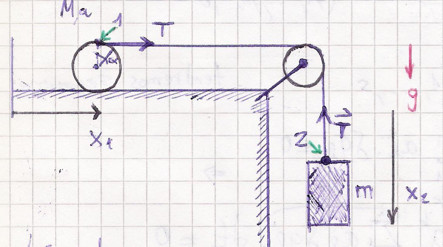
\includegraphics[scale=0.3]{images/fig_mc_cilindro_and_peso.jpg}

Los vínculos son relaciones entre velocidades que se pueden intergrar.
De la soga:
\[
	\dot{x}_1 + \dot{\alpha} a = \dot{x}_2
\]
por el rozamiento sobre el piso:
\[
	\dot{\alpha} a = \dot{x}_1
\]
\notamargen{Lo de los $\delta$ pide para ser explicado y entendido.}
\[
	\Delta x_1 + a \Delta \alpha = \Delta x_2
	\qquad \qquad 
	\Delta \alpha a = \Delta x_1
\]
\[
	\delta x_1 + a \delta \alpha - \delta x_2 = 0
	\qquad \qquad \delta x_1 - a \delta \alpha = 0 
\]
El lagrangiano es
\[
	\Lag = \frac{1}{2} m \dot{x}_2^2 + \frac{1}{2}M\dot{x}_1^2 + \frac{1}{2}I\dot{\alpha}^2 + mgx_2
\]
donde los dos términos centrales en el rhs son la cinética del cuerpo rígido.

Ahora hacemos 
\[
	\lambda^1 ( \delta x_1 + a \delta \alpha - \delta x_2 ) = 0 \qquad \qquad 
	\lambda^2 ( \delta x_1 - a \delta \alpha ) = 0
\]
donde deberíamos obtener $ \lambda^1 $ tensión y $ \lambda^2 $ fuerza de rozamiento.
Luego,
\begin{eqnarray*}
	m\ddot{x}_1 & = (\lambda^1 1 + \lambda^2 1) \\
	m\ddot{x}_2 & = mg + \lambda^1(-1) \\
	I\ddot{\alpha} & = (\lambda^1 a - \lambda^2 a)
\end{eqnarray*}

Escribiendo las ecuaciones de Newton para este problema resulta en
\begin{eqnarray*}
	m\ddot{x}_1 & = T - F_{\text{roz}} \\
	m\ddot{x}_2 & = mg - T \\
	I\ddot{\alpha} & = T a + F_{\text{roz}} a 
\end{eqnarray*}
de manera que identificamos naturalmente a 
\[
	\lambda^1 = T \qquad \qquad \lambda^2 = - F_{\text{roz}}
\]
\end{ejemplo}
% ~~~~~~~~~~~~~~~~~~~~~~~~~~~~~~~~~~~~~~~~~~~~~~~~~~~~~~~~~~~~~~~~~~~~~~~~~~~~~~~~~~~~~~~~~
% ~~~~~~~~~~~~~~~~~~~~~~~~~~~~~~~~~~~~~~~~~~~~~~~~~~~~~~~~~~~~~~~~~~~~~~~~~~~~~~~~~~~~~~~~~

Entonces, para el caso de vínculo holónomos tendremos $ a^k_\ell(q_i,t) = \nabla_i f^k \cdot \delta \vb{x}_i $ de modo que
\be
	\frac{d}{dt}\left( \dpar{\Lag}{\dot{q}_j} \right) -\dpar{\Lag}{q_j} =
	\sum_{k}^s \lambda^k \: \dpar{f^k}{q_j}
	\label{ecs_el_vinculos}
% 	\nabla_j f^k \cdot \frac{\delta \vb{x}_j}{\delta q_j}
\ee
\notamargen{Hay que escribir bien la conversión de $\nabla f^k$ hacia $\partial f^k / \partial q_j $. Parece una boludez,
pero tal vez no sea así.}

Pero sabemos [sí?] que cuando existe fuerza generalizada (no proveniente de un potencial) se tenía 
\be
	\frac{d}{dt}\left( \dpar{\Lag}{\dot{q}_j} \right) -\dpar{\Lag}{q_j} = Q_j, \qquad \qquad 
	Q_j = \sum_i^N \vb{F}_i^a \cdot \dpar{\vb{x}_i}{q_j}
	\label{ecs_el_fuerza_generalizada}
\ee
% siendo $\nabla_j f^k $ el gradiente de la ecuación de víngulo respeco de $j$ y 
e igualando los miembros derechos de \eqref{ecs_el_vinculos} y \eqref{ecs_el_fuerza_generalizada} 
\[
	\sum_i^N \vb{F}_i^a \cdot \dpar{\vb{x}_i}{q_j} = \sum_{k}^s \lambda^k \: \dpar{f^k}{q_j}
\]
se arriba a que 
\notamargen{Acá hay temas con los índices y con lo que se suma. Parece no ser la misma cosa.
Tenía observado en la carpeta que $\vb{x}=\vb{x}(q_i,t)$ y $f(q_i,t)=0$.}
\[
	\lambda^k = \vb{F}_i^a 
\]
de manera que $\lambda^k$ son las fuerzas de vínculo asociadas a los vínculos que no se pudieron retirar
(no despejados en las ecuaciones [?]).
Si los vínculos son holónomos (pero no quise despejar) entonces son las fuerzas de vínculo.

La moraleja es que si no puedo despejar en función de coordenadas independientes sí o sí necesito introducir
multiplicadores de Lagrange.

Tenía anotado que \eqref{ecs_el_fuerza_generalizada} es el lagrangiano con fuerzas no conservativas, cuando por 
supuesto $\vb{F}$ son fuerzas no conservativas.


\subsubsection{Más sobre el asunto de vínculos}
\notamargen{Hay que revisar bien esta sección y meter algún ejemplo esclarecedor.}

comparando vemos que 
\[
	Q_j = \sum \lambda^k a^k_j(q_j,t) \quad \textrm{vínculos no holónomos}
\]
\[
	Q_j=  \sum \lambda^k \nabla_j f^k \cdot \delta \vb{r}_j  \quad \textrm{vínculos holónomos}
\]

En el caso de vínculos holónomos 
\[
	g(\vb{r}_1,...,\vb{r}_n,t) = 0 
\]
donde no quise despejar en función de $q_q,...,q_n$ resulta que 
\notamargen{El supraíndice con $\delta q_j$ va sobre el igual en realidad.}
\[
	Q_j^{\delta q_j} =  \sum_i^N \lambda (\nabla_i f^k\cdot\delta\vb{r}_i)
\]
donde $\delta\vb{r}_i$ es un desplazamiento virtual de la partícula.
Vamos a reescribir este término,
\[
	\sum_i^N \dpar{g^k}{\vb{r}_i} \delta \vb{r}_i = 0
\]
\[
	\nabla_i f^k\cdot\delta\vb{r}_i = \sum_i \dpar{g^k}{\vb{r}_i} \dpar{\vb{r}_i}{q_j} \delta q_j
\]
\[
	Q_j^{\delta q_j} =  \lambda \sum_k \dpar{g^k}{\vb{r}_i} \sum_j \dpar{\vb{r}_i}{q_j} \delta q_j
\]
luego como 
\[
	a^k_j \equiv \dpar{g^k}{\vb{r}_i}
\]
se sigue que los $\lambda^k$ son las fuerzas de vínculo.

En el caso de vínculos no holónomos $\lambda^k$ son las fuerzas de vínculo asociadas a los 
vínculos no retirados.

\[
	Q_j {\delta q_j} =  \sum \lambda^k (\nabla_i g^k\cdot\delta\vb{r}_i)
\]
\[
	Q_j =  \sum_k \lambda^k \dpar{g^k}{\vb{r}_i} \dpar{\vb{r}_i}{q_j}
\]
\[
	Q_j =  \sum_k \lambda^k \dpar{g^k}{q_j}
\]
entonces $\lambda^k=F^v$.

Como extra escribamos que para cada grado de libertad $j$ 
\[
	\dpar{\Lag}{q_j} - \frac{d}{dt}\left( \dpar{\Lag}{\dot{q}_j} \right) - \sum_k^s \lambda^k a_j^k \equiv 0
\]
donde $\delta q_j$ son ahora independientes.
\[
	Q_j = \sum_i^N F_i^a \dpar{\vb{r}_i}{q_j}. 
\]

\begin{ejemplo}{\bf Moneda rodando por un plano}

Consideramos una moneda que rueda libremente por un plano (no sujeta a potencial).
Situraemos un sistema de ejes sobre la moneda, que etiquetaremos 123 y otro fijo fuera
de la misma xyz.
\[
	\vb{V}_{cm} = -\vb{\Omega} \times \vb{r} =
	-(\dot{\phi}\hat{2} + \dot{\psi}\hat{3}) \times (-a\hat{2})
\]
\[
	\dot{x}\hat{x} + \dot{y}\hat{y} = -a \dot{\psi}\hat{1}
\]
siendo los vínculos
\[
	z_{cm} - a = 0 \qquad \theta=\pi/2 \qquad |\vb{V}_{cm}| = a\dot{\psi}
\]
de tal modo que son dos grados de libertad. Los vínculos provienen de la rodadura y de considerar que la moneda 
permanece en todo momento vertical, aunque pueda cambiar la dirección de su velocidad. En este problema se deben 
utilizar multiplicadores de Lagrange de manera obligada.
El lagrangiano puede escribirse como 
\[
	\Lag = T = \frac{1}{2}m a^2 \dot{\psi}^2  + \frac{1}{2} I_2^2 \dot{\phi}^2 + \frac{1}{2} I_3^2\dot{\psi}^2.
\]
\notamargen{No entiendo/recuerdo lo que quise decir con la expresión {\it bajar los ejes}.
Calculo que se relaciona con la proyección de los ejes 123 en xyz. Confirmarlo.}

\begin{figure}
	\begin{center}
	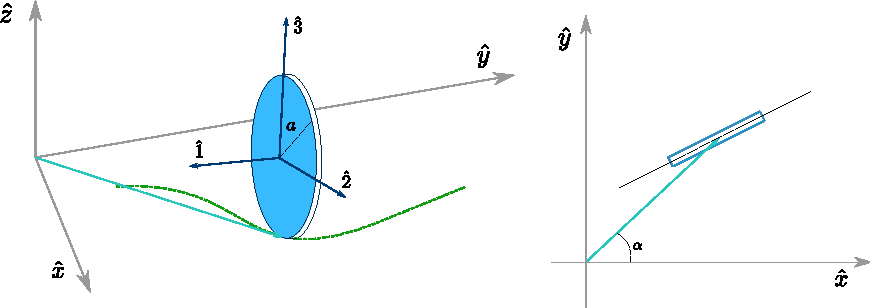
\includegraphics[width=1.0\textwidth]{images/fig_moneda.pdf}	 
	\end{center}
	\caption{Moneda que rueda libremente por un plano. Intercambié ejes 2 y 3 respecto del dibujo anterior.}
\end{figure} 

Como los vínculos dependen de la velocidad, resulta 
\[
	\dot{y} = a\dot{\psi} \cos(\psi) \sin(\phi) = a \sin(\phi) \dot{\psi}
\]
\[
	\dot{x} = a\dot{\psi} \cos(\psi) \cos(\phi) = a \cos(\phi) \dot{\psi}
\]
de tal manera que 
\[
	\dot{y} - a \sin(\phi) \dot{\psi} = 0 \qquad \dot{x} - a \cos(\phi) \dot{\psi} = 0
\]
y luego esto equivale a 
\[
	\lambda_1(dy - a \sin(\phi) d\psi) = 0 \qquad \lambda_2(dx - a \cos(\phi) d\psi)= 0
\]
y finalmente 
\[
	\frac{d}{dt}\left(\dpar{\Lag}{\dot{q}_i}\right) - \dpar{\Lag}{q_i} =
	\lambda_i \nabla_i f \cdot \delta \vb{r}_i
\]
Podemos escribir
\[
	m \ddot{x} = \lambda_1 \qquad m \ddot{x} = m a \frac{d}{dt}( \cos(\phi)\dot{\psi} )
\]
\[
	m \ddot{x} = m a ( -\sin(\phi)\dot{\phi}\dot{\psi} + \cos(\phi)\ddot{\psi} )
\]
\[
	m \ddot{y} = \lambda_2
\]
\[
	I_2\ddot{\phi} = 0 \qquad I_3\ddot{\psi} = - \lambda_2 a \sin(\phi) -\lambda_1 a \cos(\phi)
\]
\[
	\hat{1} = \cos(\psi)[\sin(\phi)\hat{y} + \cos(\phi)\hat{x}]
\]

\label{moneda}
\end{ejemplo}


\subsection{Soluciones aproximadas}

Puedo tomar un subconjunto pequeño de funciones y restringirme a buscar cua es la mejor función de ese conjunto
en el sentido de extremar $I$:
\[
	I = \int_{t_i}^{t_f} \Lag(q_1,...,q_n,\dot{q}_1,...,\dot{q}_n,t) \: dt,
\]
donde el subconjunto de las funciones $q_1,q_2, ... ,q_n$ las tomo de algún subconjunto en particular.
Por ejemplo,
\[
	q_1^f = a_0 + a_1 t_f + ... \qquad q_1^i = a_0 + a_1 t_i + ...
\]

\subsection{Oscilador armónico}

Considero un oscilador armónico en una dimensión.
\[
	\Lag = \frac{1}{2} m \dot{x}^2 - \frac{1}{2} k \dot{x}^2
\]

Quiero resolver de manera aproximada el oscilador armónico y ver que está bien.
Si considero $ n \to \infty $ tengo infinitos parámetros y puedo parametrizar cualquier curva que una los puntos
inicial y final.

\begin{figure}
	\begin{center}
	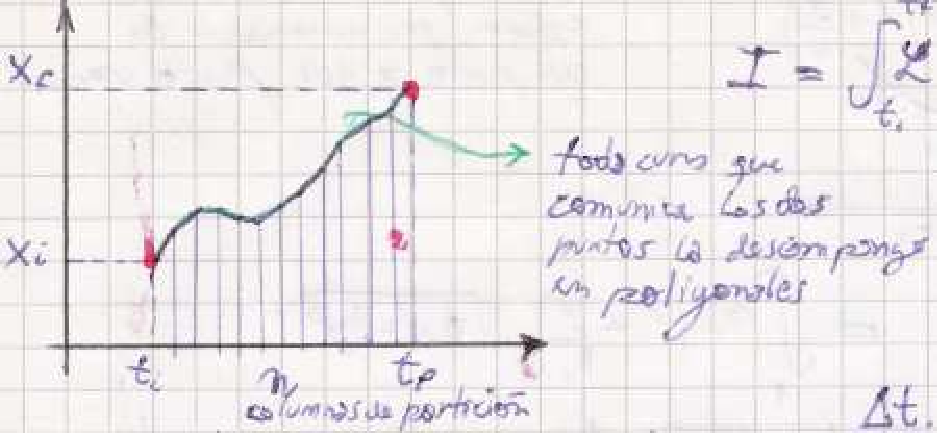
\includegraphics[scale=0.5]{images/fig_mc_oscarm_approx.pdf}	 
	\end{center}
	\caption{}
	\label{fig_mc_oscarm_approx}
\end{figure} 

\notamargen{
comments del gráfico: toda curva que comunica los dos puntos la descompongo en poligonales. Columnas de partición
}

\[
	I = \int_{t_i}^{t_f} \Lag(x,\dot{x}) \: dt
\]
Parto el intervalo y considero una partición de $N$ {\it cachos}.
\[
	\Delta t N = t_i - t_f
\]
donde $\Delta t \to 0$ y $N \to \infty $. Luego la versión discreta de la integral es 
\[
	I \approx \sum_{i=1}^{N-1} \left( \frac{1}{2}m \frac{(x_{i+1} - x_i)^2}{\Delta t^2} 
	- \frac{1}{2} k x_i^2 \right) \Delta t
\]

Tomamos la derivada
\[
	\dpar{I}{x_j} = \left( m \frac{(x_j - x_{j-1})}{\Delta t^2} - m \frac{(x_{j+1} - x_j)}{\Delta t^2} \right) 
	\Delta t - kx_j \Delta t
\]
e igualándola a cero,
\[
	\frac{m}{\Delta t^2} ( -2x_j + x_{j-1} + x_{j+1}) + k x_j = 0
\]
\notamargen{Creo que se puede usar que uno conoce diferencias finitas algo.
El final parece no estar muy claro en la carpeta. Hacer la cuenta a mano bien.}
que se puede escribir como 
\[
	\frac{m}{\Delta t}\left( \frac{x_{j+1} - x_j}{\Delta t} - \frac{x_j - x_{j-1}}{\Delta t} \right) + k x_j = 0
\]
y que en el límite continuo va a 
\[
	m\ddot{x} - kx = 0.
\]



\begin{ejemplo}{\bf Geodésicas}
\notamargen{Este material es parte de una clase práctica. Habría que ver de hacerlo encajar mejor.}
% \section{Geodésicas}
La idea es extremizar la distancia entre dos puntos de una dada geometría.
En el caso del plano se tiene 
\[
	I = \int ds = \int \sqrt{ dx^2 + dy^2 } = \int \sqrt{ 1 + \dot{y}^2 } \; dx
\]
donde se ha definido $\dot{y} \equiv dy/dx$. Evidentemente si la geometría es plana,
la curva que extremiza el intervalo tiene que ser una recta. Veámoslo.
Las ecuaciones de Euler Lagrange se reducen a:
\[
	\dtot{}{dx}\left( \frac{\dot{y}}{\sqrt{1 + \dot{y}^2 }}\right) = 0,
\]
las cuales nos dicen que 
\[
	\frac{\dot{y}}{\sqrt{1 + \dot{y}^2 }} = C
\]
donde $C$ es una constante. No es difícil ver que esta ecuación lleva a 
\[
	y(x) = C_1 x + C_2
\]
para $C_1, C_2$ constantes. Esta es la ecuación de una recta en el plano.


{\bf Un ejemplo más sofisticado}

Si a una curva $z=z(x)$ como la que se ilustra en la figura se la hace girar en torno al
eje $z$ se tiene una superficie de revolución. Un punto tridimensional en esa superficie
se puede parametrizar en términos de coordenadas cilíndricas $\rho,\theta, z$ según
\[
	\begin{cases}
	x = \rho(z) \: \cos( \theta ) \\ 
	y = \rho(z) \: \sin( \theta ) \\
	z = z
	\end{cases}
\]
donde el hecho de que la superificie es 2D se trasluce en que cada coordenada cartesiana
3D $x,y,z$ depende a lo sumo de dos variables $\theta,z$.

La trayectoria mínima entre dos puntos provendrá otra vez de extremar
\[
	I = \int ds = \int \sqrt{ dx^2 + dy^2 + dz^2 }
\]
pero utilizando la restricción de la superficie dada por las ecuaciones XXX. Utilizando
la prima para denotar la derivada con respecto a $z$ se tiene 
\[
	dx = \rho' \cos \theta dz - \rho \sin \theta d\theta
\]
\[
	dy = \rho' \sin \theta dz + \rho \cos \theta d\theta
\]

\[
	I = \int \sqrt{ {\rho'}^2 dz^2 + \rho^2 d\theta^2 + dz^2 }
\]
que se puede poner en términos de la derivada con respecto a $z$ sacando como factor común
su diferencial. Entonces
\[
	I = \int \sqrt{ ( {\rho'}^2 + 1 ) dz^2 + \rho^2 {\theta'}^2 } dz
\]
donde tanto $\rho$ como $\theta$ son funciones de $z$.
El lagrangiano es función de $\theta', \rho, \rho'$

Si calculamos las ecuaciones de Euler Lagrange para $\theta$ (que son las más fáciles puesto que
la dependencia es solo de la derivada) se llega a
\[
	\frac{\rho \rho' \theta' }{\sqrt{ ( {\rho'}^2 + 1) + \rho^2 {\theta'}^2 }} = C
\]
que se puede, haciendo el álgebra correspondiente, lleva a la forma explícita
\be
	\theta(z) = C_1 \int \frac{\sqrt{ {\rho'}^2 + 1 }}{ 2 \sqrt{ \rho^2 - C_1^2 } } dz + C_2,
	\label{ec_sup_rev}
\ee
que es una ecuación genérica para una superficie en rotación. Es decir, que recorrer la curva
de longitud mínima por esa superficie debe hacerse avanzando en $\theta$ según la prescripción
dada por \eqref{ec_sup_rev}.

Si la superficie fuera un cilindro, de radio $a$, por ejemplo, se tendría $\rho=a$ de modo que la
\eqref{ec_sup_rev} se integra inmediatamente para dar 
\[
	\theta(z) = C_1 \frac{z}{ a \sqrt{ a^2 - C_1^2 } } .
\]
Luego, para dos puntos separados verticalmente una distancia $h$ (ver figura) sobre la superficie
del cilindro se tiene que la curva que representa la distancia mínima es una hélice en el cilindro,
de paso $h$. Si la superficie lateral de este cilindro se desplegase sobre un plano, esa curva es
una recta.

{\bf Superficie general en 3D}

Si la partícula debe {\it caminar} en la superficie $\Omega$ entonces tal vez se pueda expresar
como $z=z(x,y)$ de tal forma se tendrá
\[
	I = \int f(\dot{x},\dot{y},\dot{z}) dt
\]
Luego, la derivada total de $z$ será
\[
	\dtot{z}{t} = \dot{z} = \dpar{z}{x} \dot{x} + \dpar{z}{y} \dot{y}
\]
y entonces 
\[
	I = \int f(\dot{x},\dot{y},\dpar{z}{x} \dot{x} + \dpar{z}{y} \dot{y}) dt.
\]

Planteando las ecuaciones de Euler-Lagrange 
\[
	\dtot{}{t}\left( \dtot{f}{\dot{x}} + \dtot{f}{\dot{z}}\dtot{z}{x} \right) -
	\dtot{f}{\dot{z}}\dtot{}{x}
	\left( \dpar{z}{x} \dot{x} + \dpar{z}{y} \dot{y} \right) = 0
\]
\[
	\dtot{}{t}\left( \dtot{f}{\dot{y}} + \dtot{f}{\dot{z}}\dtot{z}{y} \right) -
	\dtot{f}{\dot{z}}\dtot{\dot{z}}{y} = 0
\]
las cuales se pueden simplificar usando la derivada total,
\[
	\dtot{}{t}\left( \dtot{f}{\dot{x}} \right) + \dtot{}{t}\left( \dtot{f}{\dot{z}} \right)
	\dtot{z}{x} + \dtot{f}{\dot{z}}\dtot{}{t}\left( \dtot{z}{x} \right) + 
	\dtot{f}{\dot{z}}\dtot{}{t}\left( \dtot{z}{x} \right) = 0
\]
\notamargen{Los dos últimos términos tienen que aparecer tachados.}

Luego,
\[
	\dtot{}{t}\left( \dtot{f}{\dot{x}} \right) + 
	\dtot{z}{x}\dtot{}{t}\left( \dtot{f}{\dot{z}} \right) = 0
\]
\[
	\dtot{}{t}\left( \dtot{f}{\dot{y}} \right) + 
	\dtot{z}{y}\dtot{}{t}\left( \dtot{f}{\dot{z}} \right) = 0
\]
y como
\[
	\dtot{G}{x}\dot{x} + \dtot{G}{y}\dot{y} + \dtot{G}{z}\dot{z} = 0,
\]
se sigue que 
\[
	\dot{z} = -\left( \dtot{G}{x}\dot{x} + \dtot{G}{y}\dot{y} \right) \frac{1}{dG/dz}
\]
o bien
\[
	\dot{z} = -\left( \frac{G_x}{G_z}\dot{x} + \frac{G_y}{G_z}\dot{y} \right)
\]
de tal manera que 
\[
	\dtot{}{t}\left( \dtot{f}{\dot{x}} \right) + 
	\frac{G_x}{G_z}\dtot{}{t}\left( \dtot{f}{\dot{z}} \right) = 0
\]
\[
	\dtot{}{t}\left( \dtot{f}{\dot{y}} \right) + 
	\frac{G_y}{G_z}\dtot{}{t}\left( \dtot{f}{\dot{z}} \right) = 0
\]
\[
	\dtot{}{t}\left( \dtot{f}{\dot{z}} \right) = \lambda(t) G_z
\]

Entonces
\[
	\frac{1}{G_x} \dtot{}{t}\left( \dtot{f}{\dot{x}} \right) = 
	\frac{1}{G_y} \dtot{}{t}\left( \dtot{f}{\dot{y}} \right) = 
	\frac{1}{G_z} \dtot{}{t}\left( \dtot{f}{\dot{z}} \right) 
\]

Esta expresión puede simplificarse como 
\[
	f = \sqrt{ \dot{x}^2 + \dot{y}^2 + \dot{z}^2 } = 1
\]
si el parámetro $t$ es $s$
\[
	s = \int ds = \int \sqrt{dx^2 + dy^2 + dz^2 } =
	\int \sqrt{ \dot{x}^2 + \dot{y}^2 + \dot{z}^2 } ds
\]
y entonces
\[
	\dtot{}{t}\left( \dtot{f}{\dot{x}} \right) = \ddot{x}
\]
de manera que la ecuación de la geodésica es
\[
	\frac{1}{G_x}\dtot[2]{x}{s} = \frac{1}{G_y}\dtot[2]{y}{s} = 
	\frac{1}{G_z}\dtot[2]{z}{s}
\]

Ahora, si consideramos
\[
	I = \int [f(\dot{x}, \dot{y}, \dot{z}) + \lambda G(x,y,z)] dt
\]
se tiene que 
\[
	\dtot{}{t}\left( \dtot{f}{\dot{x}}\right) - \lambda G_x = 0
\]
y es un vínculo que hay que integrar, y es mucho más difícil.

Volviendo a la superficie general
\[
	I = \int \left[\frac{1}{2} m (\dot{x}^2 + \dot{y}^2 +
	   \dot{z}^2 ) - \lambda G \right] dt
\]
\[
	T = \sqrt{(\dot{x}^2 + \dot{y}^2 + \dot{z}^2)} = cte. \equiv k
\]
y entonces $s=kt$

\[
	k^2 m \ddot{x} - \lambda G_x = 0
\]
\[
	k^2 m \ddot{y} - \lambda G_y = 0
\]
\[
	k^2 m \ddot{z} - \lambda G_z = 0
\]

\[	
	G(x,y,z) = 0
\]

La partícula se mueve en una geodésica 
\[
	\frac{\ddot{x}}{G_x} = \frac{\ddot{y}}{G_y} = \frac{\ddot{z}}{G_z}
\]
\end{ejemplo}


% =================================================================================================
\section{Potenciales dependientes de la velocidad}
% =================================================================================================

Hasta el momento se consideró que el potencial $V$ dependía únicamente de la posición y resultaba eso en
una fuerza generalizada [la llamé así?]
\[
	Q_j = -\dpar{V}{q_j}
\]
para la cual el $\Lag\equiv T-V$ cumplía las ecuaciones de Euler Lagrange
\be
	\dtot{}{t} \left( \dpar{\Lag}{\dot{q}_j} \right) - \dpar{\Lag}{q_j} = 0.
	\label{el-pot-x}
\ee

Si en cambio se tiene un potencial dependiente, además, de la velocidad,
\[
	U = U(q_1, ..., q_2,\dot{q}_1,...,\dot{q}_n,t ) 
\]
y se requiere que sigan valiendo las ecuaciones \eqref{el-pot-x} para $\Lag \equiv T-U$, necesitaremos evidentemente
\[
	Q_j = \dtot{}{t} \left( \dpar{U}{\dot{q}_j} \right)  -\dpar{U}{q_j},
\]
una fuerza generalizada que depende de posiciones y velocidades.

El ejemplo canónico de una tal fuerza es la fuerza de Lorentz, que es la que sufre una partícula de carga $q$ en
presencia de un campo electromagnético dado por campos $\vb{E}, \vb{B}$ y cuya forma es
\be
	\vb{F} = q \vb{E} + \frac{q}{c} ( \vb{v} \times \vb{B} )
	\label{f_lorentz}
\ee

Esta fuerza \eqref{f_lorentz} puede expresarse en términos de dos potenciales. Para ello es necesario recurrir a
las relaciones que verifican los campos $\vb{E}, \vb{B}$ y que están dadas por las ecuaciones de Maxwell, cuyo esquema 
se presenta en la siguiente tabla.
\begin{center}
\begin{tabular}{|c|c|}
\hline
& \\
$ \nabla\cdot\vb{E} = 4 \pi \rho $ & $ \nabla \cdot \vb{B} = 0 $ \\
& \\
$ \displaystyle \rotorm{E} = -\frac{1}{c} \dpar{\vb{B}}{t} $ &  
$ \displaystyle \rotorm{B} = \frac{4\pi}{c}\vb{J} + \frac{1}{c} \dpar{\vb{E}}{t} $ \\
 & \\
\hline
\end{tabular}
\end{center}

Dado que la divergencia de \vb{B} es nula, entonces existe un potencial vector \vb{A} tal que 
\[
	\rotorm{A} = \vb{B}.
\]
Entonces, la ley de Faraday resulta 
\[
	\rotorm{E} = -\frac{1}{c} \dpar{}{t} \left(\rotorm{A} \right) 
\]
o bien 
\[
	\nabla\times\left( \vb{E} + \frac{1}{c}\dpar{\vb{A}}{t} \right) = 0
\]

La cantidad entre paréntesis es de rotor nulo y entonces se puede escribir
\[
	\vb{E} + \frac{1}{c}\dpar{\vb{A}}{t} = -\nabla \vp( \vb{x}, t )
\]
de manera que los campos \vb{B}, \vb{E} pueden expresarse en términos de una función escalar $\vp$ y un campo vectorial
\vb{A} como
\[
	\vb{B} = \rotorm{A} \qquad \qquad \vb{E} = - \nabla \vp - \frac{1}{c} \dpar{ \vb{A} }{t} .
\]

Entonces, en términos de estos potenciales \eqref{f_lorentz} resulta 
\[
	\vb{F} = -q\nabla \vp - \frac{q}{c} \dpar{ \vb{A} }{t} + \frac{q}{c} \vb{v} \times \rotorm{A}.
\]

Supongamos, para simplificar el razonamiento, que es $ \vb{F} = F_x \hat{x} $ y veamos que 
\[
	F_x = -q \dpar{ \vp }{ x } - \frac{q}{c} \dpar{ A_x }{t} + \frac{q}{c} \left( v_y [\rotorm{A}]_z - v_z [\rotorm{A}]_y \right)
\]
se puede escribir
\[
	F_x = \dtot{}{t} \left( \dpar{U}{v_x} \right)  -\dpar{U}{x}.
\]

Desarrollando explícitamente el rotor se tiene 
\[
	\left( v_y [\rotorm{A}]_z - v_z [\rotorm{A}]_y \right) = 
	v_y \dpar{A_y}{x} - v_y \dpar{A_x}{y} - v_z \dpar{A_x}{z} + v_z \dpar{A_z}{x} + v_x \dpar{A_x}{x} - v_x \dpar{A_x}{x}
\]
donde se ha sumado y restado la conveniente combinación $ v_x \partial_x A_x $. Dado que las velocidades y las posiciones son variables
independientes (se verifica $ \partial_a v_b = 0 $ para cualquier combinación $ a,b=x,y,z $) se puede {\it filtrar} la velocidad dentro
de las derivadas para reescribir 
\[
	v_x \dpar{A_x}{x} + v_y \dpar{A_y}{x} + v_z \dpar{A_z}{x} = \dpar{}{x}( v_xA_x + v_yA_y + v_zA_z ) = \dpar{}{x}( \pe{v}{A} )
\]
% \[
% 	\left( v_y [\rotorm{A}]_z - v_z [\rotorm{A}]_y \right) = 
% 	\dpar{}{x}( v_xA_x + v_yA_y + v_zA_z ) - v_x\dpar{ A_x}{x} - v_y\dpar{A_x}{y} - v_z\dpar{A_x}{z}.
% \]
Los tres términos restantes en derivadas respecto de $A_x$ no son otra cosa que una derivada total,
\[
	- \frac{q}{c} \left(  \dpar{ A_x }{t}- v_x\dpar{ A_x}{x} - v_y\dpar{A_x}{y} - v_z\dpar{A_x}{z} \right) =
	- \frac{q}{c} \left( \dpar{ A_x }{t} - \vb{v}\cdot\nabla( A_x ) \right) = - \frac{q}{c} \dtot{A_x}{t}
\]

Luego, se fuerza la aparición de una derivada con respecto a la velocidad (para obtener una expresión en consonancia con la buscada)
del siguiente modo
\[
	A_x = \dpar{}{v_x}(v_xA_x + v_yA_y + v_zA_z) = \dpar{}{v_x}(\pe{v}{A}),
\]
y juntando todo resulta
% \[
% 	F_x = -q \dpar{ \vp }{ x } - \frac{q}{c} \dpar{ A_x }{t} + \frac{q}{c} \left( \dpar{}{x}( \pe{v}{A} )
% 	- v_i \partial_i\left( \dpar{}{v_x}(\pe{v}{A}) \right) \right)
% % 	- v_x \dpar{}{x}( \dpar{}{v_x}(\pe{v}{A}) ) - v_y \dpar{}{y}( \dpar{}{v_x}(\pe{v}{A}) ) 
% % 	- v_z \dpar{}{z}( \dpar{}{v_x}(\pe{v}{A}) ) \right).
% % 	
% \]
% donde el último término en el RHS representa la suma de tres. Reordenando esta expresión
\[
	F_x = -\dpar{ }{ x }\left( q\vp - \frac{q}{c} \pe{v}{A} \right) 
	+ \dtot{ }{t} \left( \dpar{}{v_x}\left( -\frac{q}{c}\pe{v}{A} \right) \right) .
\]

Como $\vp=\vp(\vb{x},t)$, se la puede incluir dentro de la derivada con respecto a la velocidad obteniendo finalmente el 
resultado buscado
\[
	F_x = -\dpar{ U }{ x } + \dtot{ }{t}\left( \dpar{U}{v_x} \right),
\]
donde 
\[
	U = q \vp - \frac{q}{c} \pe{v}{A}.
\]
 
\notamargen{Mucho para tener en cuenta: resumen previo de notación indicial, resumen de classical field theory. Aclarar
que posición y velocidad son independientes.}

Se puede demostrar directamente la fórmula anterior desde la expresión vectorial de \vb{F} utilizando su equivalente 
indicial, es decir a partir de
\[
	F_i = -q \partial_i \vp - \frac{q}{c} \:\partial_t A_i + \frac{q}{c} \: \epsilon_{ilm} v_l \epsilon_{mjk} 
	\partial_j A_k
\]
que es la coordenada $i$-ésima de la fuerza \vb{F}. Utilizando las propiedades del símbolo de Levi-Civita se tiene 
\[
	F_i = -q \partial_i \vp + \frac{q}{c} \left[  -\partial_t A_i  + (\delta_{ij}\delta_{lk} - \delta_{ik}\delta_{lj}) v_l \partial_j A_k \right]
\]
y, tras colapsar las deltas, y reordenar términos
\[
	F_i = -q \partial_i \vp + \frac{q}{c} \left[  -\partial_t A_i - v_j \partial_j A_i +  v_k \partial_i A_k  \right].
\]

Como el campo de velocidad \vb{v} no depende explícitamente de \vb{x} se puede introducir $v_k$ a través de la derivada $\partial_i$. Además los
dos primeros términos del corchete representan la derivada total de $A_i$ de manera que tenemos
\[
	F_i = -q \partial_i \vp + \frac{q}{c} \left[  - \dtot{}{t} \left(A_i\right)  + \partial_i (v_k A_k)  \right],
\]
o bien 
\[
	F_i = - \partial_i \left[ q\vp - \frac{q}{c}  (v_k A_k) \right] -  \dtot{}{t} \left( \frac{q}{c} A_i \right).
\]

Se puede hacer aparecer explícitamente lo faltante dentro de la derivada total notando que se puede escribir de manera absolutamente general
\[
	\frac{q}{c} A_i =  \dpar{}{v_i} ( - q\vp + \frac{q}{c} v_k A_k )
\]
dado que $\vp$ y $\vb{A}$ son funciones de la posición y el tiempo solamente. Luego,
\[
	F_i = - \partial_i \left[ q\vp - \frac{q}{c}  (v_k A_k) \right] + \dtot{}{t} \left[ \dpar{}{v_i} ( q\vp - \frac{q}{c} v_k A_k ) \right]
\]
y esto significa que el potencial completo es
\[
	U(\vb{x},\vb{v},t) = q \: \vp(\vb{x},t) - \frac{q}{c} \: \pe{v}{A}(\vb{x},t).
\]

En el ejemplo de la fuerza de Lorentz se desprecia el campo generado por la misma partícula que se mueve. Es decir, 
que el campo externo no es afectado por el movimiento de la partícula.
Una formulación lagrangiana que lo tuviera en cuenta debería considerar un $\Lag_p$ para la partícula.

% =================================================================================================
\section{Cambio de {\it gauge} en potenciales}
% =================================================================================================

Según se vio en la sección anterior, en el caso del electromagnetismo tenemos un potencial $ U $ que depende de la posición y la velocidad
de una manera muy especial. Además el potencial escalar $ \vp $ usual en la electrostática fue necesario definir un potencial vector \vb{A}
que estaba vinculado con el campo magnético \vb{B} a través de : $\rotorm{A}=\vb{B}$.

Solamente se le pide al campo \vb{A} que su rotor sea \vb{B} y esto no lo determina por completo. En particular si se define 
\[
	\vb{A}' = \vb{A} + \nabla f,
\]
un nuevo potencial $\vb{A}'$ que difiere del original por el añadido del gradiente de una función escalar, las ecuaciones de movimiento
no se ven alteradas. En efecto, la divergencia del campo magnético \vb{B} es
\[
	\divem{B} = \nabla \symbf{\cdot} (\rotorm{A}') = 
	\nabla \symbf{\cdot} (\rotorm{A}) + \nabla \symbf{\cdot} (\nabla \times {\nabla f}) = 0
\]
donde el cero se logra porque cada uno de los dos miembros es cero por separado.
Asimismo, como el rotor de un gradiente es nulo, el rotor de \vb{B} no se ve alterado;
\[
	\rotorm{B} = \nabla \times( \rotorm{A}' ) =
	\nabla \times( \rotorm{A} ) + \nabla \times ( \nabla \times \nabla f ) =
	\nabla \times( \rotorm{A} ).
\]

Luego, hay un grado de libertad extra en la determinación del \vb{A} que es esta función escalar $f$, y que se suele expresar
dando la divergencia de \vb{A}. En efecto, 
\[
	\divem{A}' = \divem{A} + \nabla^2 f.
\]

La divergencia de \vb{A} se puede elegir entonces arbitrariamente y esto es lo que se conoce como la {\it libertad de gauge}[?]
o el cambio de {\it gauge} del potencial. Descansa en el hecho de que las ecuaciones de movimiento son, por supuesto, independientes
del gauge elegido.
\notamargen{Chequear esta mini subsección.}


% Como ejemplo citamos \cite{einstein}.
% O bien \cite{example}.
% Tal vez \citep{Aspnes:1973}

% ============================================================================

% \bibliographystyle{CBFT-apa-good} % (uses file "apa-good.bst")
% \bibliography{CBFT.Referencias} % La base de datos bibliográfica


\end{document}
